\documentclass[journal=jpcbfk,manuscript=article]{achemso}

\usepackage{graphicx}
\usepackage{wrapfig}
\usepackage{subcaption}
\usepackage{amsmath} % or simply amstext
\usepackage{amssymb}
\usepackage{siunitx}
\usepackage{booktabs}
\usepackage[export]{adjustbox}
\newcommand{\angstrom}{\textup{\AA}}
\usepackage{cleveref}
\usepackage{booktabs}
\usepackage{gensymb}
\usepackage{float}
\usepackage{xr}
\usepackage{enumitem}
\newcommand{\nclusters}{10}
%\DeclareUnicodeCharacter{03C9}{$\omega$}
\externaldocument[S-]{Supporting_Information}

\SectionNumbersOn

\title{Statistical Inference of Transport Mechanisms and Long Time Scale Behavior from Time Series 
       of Solute Trajectories in Nanostructured Membranes}
\author{Benjamin J. Coscia}
\affiliation{Department of Chemical and Biological Engineering, University of Colorado Boulder, Boulder, CO 80309, USA}
\author{Christopher P. Calderon}
\affiliation{Ursa Analytics, Inc., Denver, CO 80212, USA}
\alsoaffiliation{Department of Chemical and Biological Engineering, University of Colorado Boulder, Boulder, CO 80309, USA}
\author{Michael R. Shirts}
\email{michael.shirts@colorado.edu}
\affiliation{Department of Chemical and Biological Engineering, University of Colorado Boulder, Boulder, CO 80309, USA}

\begin{document}

  \graphicspath{{./figures/}}
  \maketitle
  
  \begin{abstract}

  Appropriate time series modeling of complex diffusion in soft matter systems on the
  microsecond time scale can provide a path towards inferring transport mechanisms and
  predicting bulk properties characteristic of much longer time scales. In this work 
  we apply nonparametric Bayesian time series analysis, more specifically the sticky 
  hierarchical Dirichlet process autoregressive hidden Markov model
  (HDP-AR-HMM) to solute center-of-mass trajectories generated from long molecular dynamics (MD)
  simulations in a cross-linked inverted hexagonal phase lyotropic liquid crystal (LLC)
  membrane in order to automatically detect a variety of solute dynamical modes. 

  We can better understand the mechanisms controlling these dynamical modes by grouping 
  the states identified by the HDP-AR-HMM into clusters based on multiple metrics
  aimed at distinguishing solute behavior based on their fluctuations, dwell times
  in each state and position within the inhomogeneous membrane structure. We analyze
  predominate clusters in order to relate their dynamical parameters to physical
  interactions between solutes and the membrane. 

  Along with parameters of individual states, the HDP-AR-HMM simultaneously infers a 
  transition matrix which allows us to stochastically propagate solute behavior from 
  all of the independent trajectories onto arbitrary length time scales while still 
  preserving the qualitative behavior characteristic of the MD trajectories. This 
  affords a direct connection to important macroscopic observables used to characterize
  performance like solute flux and selectivity. 

  Overall, this work provides a promising way to simultaneously identify transport 
  mechanisms in nanoporous materials and project complex diffusive behavior on
  long time scales. Our enhanced understanding of the diverse range of solute behavior
  allows us to hypothesize design changes to LLC monomers aimed towards controlling the
  rates of solute passage, thus improving the selective performance of LLC membranes. 
  
  \end{abstract}  
  
  \section{Introduction}
  
  There is a need for highly selective membranes in order to perform efficient 
  separations of the components of complex aqueous streams. Seawater and
  brackish water desalination, separation of organic micropollutants from 
  municipal water supplies, recovery of valuable dissolved species from 
  waste streams and the creation of breathable barriers to harmful contaminants are just a
  subset of the broad range of applications for selective membrane separations.~\cite{fritzmann_state---art_2007,fonseca_couto_critical_2018,dischinger_evaluation_2019,ramaseshan_functionalized_2006}
  While researchers often focus on membrane permeability, many argue that
  it may be more beneficial to focus on membrane selectivity in order to 
  reduce the costs of commercial nanofiltration and reverse osmosis.~\cite{werber_materials_2016}
  
  The ability to efficiently design novel membrane materials for selective separations 
  would be greatly enhanced by easily interpretable methods for connecting microscopic
  fluctuations with macroscopic observables. If one can use molecular dynamics (MD)
  simulations to explain important experimental metrics such as solute flux and 
  selectivity in terms of detailed chemically dependent solute motion, then we can 
  more easily bridge the disconnect between theory and application. In many simple 
  systems, short-time scale dynamics and large scale properties can be connected by
  the simple relationship between the mean square displacement (MSD) of the solutes
  and the macroscopic diffusion constant. However, for systems which exhibit complex 
  short timescale subdiffusive dynamics, one cannot reliably compute diffusion 
  constants because MSDs are often non-linear on the timescales accessible to molecular
  simulation. Additionally, direct calculations of diffusion constants may obscure the
  molecular mechanisms controlling transport, hindering the ability to understand or 
  modulate these mechanisms in new membrane materials. We are therefore in need of a 
  more flexible approach for modeling solute dynamics which makes less assumptions 
  about the solute's short time scale behavior.

  In this work, we are particularly interested in the design of lyotropic liquid 
  crystal (LLC) monomers, a class of amphiphilic molecules whose ordered self-assembled
  phases can be cross-linked into mechanically strong membranes capable of highly 
  selective separations. Inverted hexagonal phase, or H\textsubscript{II}, LLC membranes
  are synthesized with 10 \% water by weight and are characterized by hexagonally packed,
  uniform-sized and straight pores, an ideal geometry for high throughput transport. 
  Their pores are lined with the LLC monomer's functional groups which can potentially 
  be designed to interact with solutes in a chemically-specific manner. It would be 
  extremely useful to experimentalists if we could connect LLC monomer design with 
  measurable quantities such as diffusivity and selectivity.
  %r1_comment4
  In many systems, including LLC membranes with higher water contents, making this 
  connection is a relatively straightforward calculation since small solutes and water
  can move relatively unimpeded and therefore enter a diffusive regime on timescales
  accessible to MD. When possible, we encourage the reader to take advantage of the
  simplest approach possible.
  However, in the systems of interested to us,
  this goal is complicated by the non-Brownian hopping and trapping behavior induced by the membrane's diverse
  topology and inhomogeneous structure resulting in subdiffusive behavior out to 
  multiple microseconds of simulation.~\cite{coscia_understanding_2019,coscia_chemically_2019}
  
  %r1_comment2
  A number of approaches have been explored to inexpensively extend the relatively short
  trajectories output by molecular simulations which exhibit complex diffusive behaviors
  onto much longer timescales. The trajectory extending kinetic Monte Carlo (TEKMC) approach
  divides a unit cell into a three dimensional grid and quantifies the transition 
  probabilities of particles that can move between each subdivision allowing one to generate
  stochastic trajectories that reach the diffusive regime~\cite{neyertz_trajectory-extending_2010}
  It is possible to parameterize TEKMC models with relatively short simulation trajectories 
  which facilitates systematic studies of small perturbations to material constituents.~\cite{hanson_computer_2012}
  In a related approach, dynamic bond percolation (DBP) theory can be used to quantify the
  rate of transition between sites in a dynamically disordered medium and long timescale
  behavior can be propagated using kinetic Monte Carlo simulations.~\cite{druger_dynamic_1983}
  Webb et al. extended this approach by defining sites based on the molecular details of 
  a polymer electrolyte system, thus allowing them to explain ion diffusivities predicted by
  the model in terms of chemically specific interactions.~\cite{webb_chemically_2015}

%  We have already advanced our understanding of LLC monomer design in our previous work
%  by building stochastic time series models based on the chemical intuition gained
%  from qualitative MD studies of solute transport in an H\textsubscript{II} phase LLC
%  membrane.~\cite{coscia_chemically_2019,coscia_capturing_2020} 
  Based on the chemical intuition gained from our previous qualitative MD studies of 
  solute transport in an H\textsubscript{II} phase LLC membrane, we have contributed our
  own stochastic modeling approaches with goals similar to both TEKMC and DBP.~\cite{coscia_chemically_2019,coscia_capturing_2020}
  We identified three classes of trapping behavior which result in subdiffusion out to the microsecond 
  time scale. In our first approach to stochastically model this behavior, we treated 
  the system's dynamics as a sequence of anti-correlated hops between power law distributed periods of 
  entrapment, a framework called subordinated fractional Brownian or L\'evy
  motion.~\cite{thiel_weak_2014,teuerle_modeling_2013} In a second approach, we treated 
  solute motion as a Markov state model~\cite{pande_everything_2010} with state-dependent
  dynamics, where we parameterized the state transition probabilities between each of
  eight discrete states, defined by the observed trapping mechanisms, as well as the 
  solute dynamics within each of these states. We showed how one could use realizations
  of any stochastic model like these in order to predict macroscopic flux and selectivity. 
  
  Although powerful and insightful, TEKMC, DBP and our previous work required considerable
  human effort in order to analyze the MD trajectories and to hypothesize stochastic models 
  which matched the behavior of solutes. It would be significantly more useful and broadly 
  applicable if we could design an approach which distinguishes and parameterizes varied
  solute dynamics in a data-driven way and leaves a facile way to generate an ensemble
  of stochastic trajectory realizations that can be used to predict macroscopic transport
  properties.
  
  In this work we attempt to uncover similar physical meaning through a data-driven process. 
  We utilize the sticky hierarchical Dirichlet process autoregressive hidden Markov model 
  (HDP-AR-HMM), a nonparameteric Bayesian classification technique that allows the user to 
  automatically detect and infer the parameters of an unknown number of latent vector
  autoregressive (VAR) modes present in solute center-of-mass MD 
  trajectories.~\cite{fox_bayesian_2010} The sticky HDP-AR-HMM greatly extends the 
  basic framework of simpler but more limited finite hidden Markov modeling approaches.
    
  In their most basic form, hidden Markov models (HMMs) are used to generate
  a series of latent, or hidden, states dependent only on the previous state.~\cite{rabiner_tutorial_1989}
  Propagating an HMM generates sequential but conditionally independent observations from 
  the emission distributions associated with each hidden state. 
  Within an HMM, dynamics (i.e. temporal dependence) are modeled solely through  
  a matrix of transition probabilities. Given a series of observations and a known number of hidden states, the 
  Baum-Welch algorithm, an expectation maximization technique, is a commonly 
  used way to determine the hidden state sequence and the underlying parameters of
  a standard HMM.~\cite{baum_maximization_1970} However, it is also possible to infer
  HMM parameters through a Bayesian framework.~\cite{scott_bayesian_2002,jasra_markov_2005} 
  One can place priors on the transition probabilities and parameters of the hidden 
  states' emission distributions in order to iteratively infer their values and to
  estimate the hidden state sequence. HMMs have been used in a broad range of applications
  including speech recognition, weather forecasting and bioinformatics.~\cite{juang_hidden_1984,hughes_non-homogeneous_1999,yoon_hidden_2009}.
  In molecular simulations, HMMs have been used to characterize molecular kinetics
  in order to determine the equilibrium distribution of various observables.~\cite{thayer_hidden_2002,singhal_using_2004,noe_probability_2008,noe_projected_2013}
  
  By placing a hierarchical Dirichlet process (HDP) prior on the observed time
  series data, it is possible to extend HMMs to an unknown number of hidden
  states, thus allowing the model's complexity to be driven by the complexity
  of the data.~\cite{teh_hierarchical_2006} We will refer to a model calibrated with
  this type of prior as an HDP-HMM; this model class is sometimes referred to
  as an infinite hidden Markov model.~\cite{beal_infinite_2002} The HDP-HMM 
  elegantly overcomes the main shortcoming of standard HMMs, the need to choose
  the number of states \textit{a priori}, making its use more advantageous in
  a diversity of applications including economic data and single particle trajectory 
  analysis.~\cite{shi_identifying_2016,hines_analyzing_2015,sgouralis_introduction_2017,jazani_alternative_2019,wang_single-molecule_2014,persson_extracting_2013} 

  One issue with the original formulation of the HDP-HMM is that it does 
  not distinguish self-transitions and transitions between different states.
  Practically, this can result in rapid switching between states and inferred
  state sequence representations that do a poor job of describing the 
  observations. Rapid state switching in the original HDP-HMM not only 
  reduces the predictive ability of the model, but in many cases is also 
  physically unrealistic and can complicate model interpretation. 
  Fox et al. addressed this issue by adding a `sticky'
  parameter.~\cite{fox_sticky_2007} The sticky HDP-HMM is useful in situations
  where the user has prior knowledge that state persistence is likely.
  For example, in the case of speaker diarization, it is unlikely that a 
  conversation between two people would rapidly switch between speakers.~\cite{fox_sticky_2011}
  This is also important for our work where we expect state persistence due
  to solute entrapment.   
  
  The utility of the sticky HDP-HMM has been further extended to account for
  inherent temporal dependence between measurements common to many time series
  datasets. For example, in both MD and single particle tracking, there is 
  strong temporal dependence/correlation between successive measurements even
  within a fixed state.~\cite{calderon_data-driven_2014}
  Fox et al. formulated a method that accounts for temporal dependence between
  successive observations by incorporating Markov jump linear systems (MJLSs)
  into infinite state models.~\cite{fox_nonparametric_2009} An MJLS models 
  each dynamical mode as a linear dynamical process. Two MJLS sub-classes are 
  switching linear dynamical systems (SLDSs) and switching vector autoregressive
  (VAR) processes. Switching VAR processes are a sub-class of SLDSs that do not
  incorporate measurement noise. Since MD simulations do not contain measurement
  noise, we will model the dynamical modes exhibited by MD solute trajectories 
  as VAR processes and we will refer to our model as an application of the 
  sticky HDP-AR-HMM in order to maintain its distinction from the even more
  general sticky HDP-SLDS models.
  
  To our knowledge, applying the HDP-AR-HMM in order to gain kinetic and
  mechanistic insight from MD simulation trajectories has not been done
  before. Typical applications of the HDP-AR-HMM center around determining the 
  number of states, the state sequence and analysis of the emission 
  distributions of a time series. The addition of temporal correlation to 
  the inference procedure has primarily been used to improve state sequence 
  identification.~\cite{calderon_inferring_2015} In our approach, we use the
  HDP-AR-HMM not only to segment a collection of MD time series into distinct 
  dynamical modes, but to uncover unknown transport mechanisms and to create 
  improved predictive models. We cluster the parameters of individual states
  in order to reduce the total state space down to an interpretable size.
  This allows us to learn the implied dominant physical mechanisms and describe
  solute kinetics based on interpretation of distinct parameters that dominate
  the ensemble of MD trajectories. We can use the model parameters determined 
  either before or after clustering to generate new time series trajectories 
  which enable projections of the MD-generated time series to arbitrary length
  time scales.
  
  % BJC: Michael prefers not to put any conclusions in the intro. So we basically pose
  % questions to which we already know the answer, with the intent of readers having
  % a better sense of what to look for while reading.
  We aim to address two primary scientific questions with this work:
  \begin{enumerate}
  
  \item First, we want to know whether it is possible to use the HDP-AR-HMM to 
  help us predict macroscopic transport properties. We use the VAR parameters
  and state transition probability matrix of the HDP-AR-HMM in order to 
  generate stochastic trajectory realizations with behavior similar to that
  exhibited by MD. One can project these realizations onto much longer 
  time scales with computational ease extending into time scales where 
  regular diffusive behavior again occurs.
  
  \item Second, we want to know if the HDP-AR-HMM algorithm can help
  efficiently uncover underlying transport mechanisms which give rise to different 
  solute dynamical behavior. We cluster states with similar parameters
  across all trajectories in order to reduce the total state space and to 
  identify which segments of the solute trajectories exhibit similar behavior. We use the 
  parameters of the clustered states identified by the HDP-AR-HMM in order to 
  infer dominant solute-membrane interactions and transport mechanisms. We 
  support our mechanistic hypotheses via quantitative comparison to various 
  physical membrane properties and solute-membrane interactions.
  
  \end{enumerate}

  \section{Methods}
    
  We ran all MD simulations and energy minimizations using GROMACS 2018.~\cite{bekker_gromacs:_1993,berendsen_gromacs:_1995,van_der_spoel_gromacs:_2005,hess_gromacs_2008}  
  We implemented the sticky HDP-AR-HMM in Python 
  (\texttt{https://github.com/shirtsgroup/hdphmm}) which we heavily adapted from
  the MATLAB code of Fox et al.~\cite{fox_nonparametric_2009} Since we do not incorporate
  any novel methodology to the HDP-AR-HMM inference procedure, we refer the 
  interested reader to an excellent and in-depth description of the formulation of
  the HDP-AR-HMM and related models.~\cite{fox_bayesian_2010} 
  All other post-simulation trajectory analysis tools are available online at
  \texttt{https://github.com/shirtsgroup/LLC\_Membranes}.

  \subsection{Molecular Dynamics Simulations}

  We studied transport of solutes in the H\textsubscript{II} phase using our
  previously developed atomistic molecular model of four pores in a $9.4\times9.4\times7.6$ nm 
  monoclinic unit cell with 10\% water by weight, totaling 62,000 atoms. Approximately
  one third of the water molecules occupy the tail region with the rest are near the
  pore center.~\cite{coscia_chemically_2019}

  %r1_comment3  
  We modeled water molecules using the TIP3P water model,~\cite{jorgensen_comparison_1983}
  We used the Antechamber module shipped with AmberTools18 to parameterize monomers and 
  solutes using the Generalized Amber Force Field (GAFF).~\cite{wang_development_2004} We 
  assigned charges using the AM1-BCC model as implemented in Antechamber.~\cite{jakalian_fast_2000,jakalian_fast_2002}
  GAFF is very commonly used in simulations with diverse organic chemical functionality, 
  and was developed for consistency within the AMBER ecosystem, which uses TIP3P as the
  water model. We chose these standard force fields and generalizable parameterization 
  approaches so that a range of solutes and monomers could be self-consistently and easily 
  studied. The main goal of this work is to develop stochastic models which can reproduce
  solute behavior on MD time scales, independent of the choice of force field. In future 
  work, it may be beneficial to employ specialized force fields, including polarizable 
  force fields or other higher-order effects in order to improve the accuracy of structure 
  parameters and selectivity predictions.
    
  We chose to study a subset of 4 of the fastest moving solutes from our previous
  work: methanol, acetic acid, urea and ethylene glycol. In addition to exploring 
  membrane structural space the most, these solutes have a relatively diverse set
  of chemical functionality. For each solute we created a separate system and to 
  each system we added 6 solutes per pore for a total of 24 solutes. This number 
  of solutes per pore provides a sufficient amount of data from which to generate 
  statistics on the time scales which we simulate and prevents any significant
  solute clustering facilitating our study of pure solute-membrane interactions. 
  Further details on the setup and equilibration of these systems are detailed 
  in our previous work.~\cite{coscia_chemically_2019}
  
  Each solute system was simulated for 5 $\mu$s using MD. We used a time step of 2 
  fs at a pressure of 1 bar and temperature of 300K controlled by the semi-isotropic 
  Parrinello-Rahman barostat~\cite{parrinello_polymorphic_1981} and velocity rescale 
  thermostat~\cite{bussi_canonical_2007} respectively. We recorded configurations every 0.5 ns.

  \subsection{Applying the sticky HDP-AR-HMM to MD Trajectories}\label{method:HDP-AR-HMM}

  We use the sticky HDP-AR-HMM in order to assign the time-correlated positional 
  fluctuations of solute center-of-mass MD trajectories to discrete dynamical modes while 
  simultaneously inferring the VAR parameters of those modes. We use the sticky model
  in order to encourage higher self-transition probabilities since we physically observe
  solute entrapment in states for appreciable amounts of time. 
  
  Although the discussion will be presented in terms of 2D cylindrical coordinates, we
  applied the HDP-AR-HMM algorithm to 3D solute center-of-mass coordinate trajectories 
  with the radial dimension represented by the solute's $x$ and $y$ coordinates 
  transformed relative to the nearest pore center, and the $z$ axis oriented along 
  the membrane pore. By working in Cartesian coordinates, we avoid mathematical 
  complexity introduced by changing into cylindrical coordinates while
  estimating the state sequence.
  
  \textit{Parameterizing the Hidden States}: We describe the dynamics of each 
  state visited by solutes in our MD simulations using a first order vector 
  autoregressive (VAR(1)) model. In general, a VAR($r$) process is characterized by a
  vector of observations in a time series that are linearly dependent on $r$ previous
  values of the time series vector:
  \begin{equation}
  	\mathbf{y}_t = \mathbf{c} + \sum_{i=1}^r A_i\mathbf{y}_{t-i} + \mathbf{e}_t~~~~\mathbf{e}_t \sim \mathcal{N}(0, \Sigma)
  \label{eqn:var}
  \end{equation}
  Previous observations are weighted by coefficient matrices, $A_i$. The VAR($r$) 
  process is further characterized by a shift in the mean of each dimension by the
  vector $\mathbf{c}$ and a white noise term $\mathbf{e}_t$.~\cite{hamilton_time_1994}
  We assumed $\mathbf{e}_t$ to be multivariate Gaussian noise, with mean zero and
  covariance, $\Sigma$. We limited our analysis to an autoregressive order of $r=1$.
  This means that we only parameterize $A_1$. To simplify notation, we will call it $A$. 
  We used a conjugate matrix-normal inverse-Wishart (MNIW) prior on parameters 
  $A$ and $\Sigma$ and a Gaussian prior on $\mathbf{c}$ in order to efficiently infer their 
  values.~\cite{fox_nonparametric_2009}
  
  \textit{State sequence and parameter inference}: We ran 2000 iterations of the
  HDP-AR-HMM procedure on each trajectory which was sufficient in order to arrive
  at converged state sequences and VAR parameter estimates. By our criteria, the 
  procedure generally converged within 500--1000 iterations. We evaluated 
  convergence based on when the VAR parameter estimates plateaued. We detected 
  plateaus using the module \\ \texttt{pymbar.timeseries.detect\_equilibration}~\cite{chodera_simple_2016} 
  on the time series of the individual parameters (see Section~\ref{S-section:convergence}
  of the Supporting Information). Convergence of the VAR parameters implies that
  the state sequence is relatively stable since the inferred parameters are 
  sensitive to the inputs to the MNIW conjugate priors. The precise boundaries of 
  the state segments can fluctuate; therefore, in states with a low number of 
  emissions, the variance in $A$ and $\Sigma$ parameters can be high. In these 
  cases, plateauing of the mean in each dimension tends to be a more reliable 
  indicator of convergence (see Figure~\ref{S-fig:convergence3d} of the Supporting
  Information).
  
  It is usually beneficial to employ well-informed state sequence initialization 
  procedures in nonparametric Bayesian approaches.~\cite{fox_bayesian_2010}
  Most importantly in this work, the states identified by the HDP-AR-HMM are heavily 
  influenced by the Gaussian prior placed on $\mathbf{c}$ in Equation~\ref{eqn:var}. In 
  Section~\ref{S-section:fitting_tips} of the Supporting Information we outline our 
  algorithmic method for choosing reliable prior parameters in addition to other 
  practical tips for initialization.

  We inferred the state sequence and parameters for each of the 24 solute 
  trajectories independently. Although the HDP-AR-HMM is capable of identifying 
  an infinite number of states, a Dirichlet process exhibits a ``rich get richer" 
  effect, favoring a fewer number of states.~\cite{dreyer_discovering_2011}
  By applying the algorithm to each trajectory independently, we reduce the 
  possibility of lumping together multiple similar, but distinct states. In 
  Section~\ref{method:realizations}, we explain how we use these 24 independent
  models in order to generate a single MSD prediction.  
  
  \subsection{State Clustering}\label{method:clustering}  

  We clustered states with like parameter sets in order to reduce the state space to
  a more easily interpretable size and because the parameters of a single state 
  alone does not always have enough context to provide meaningful physical insight.
  For each solute studied, we identified approximately 300-500 independent states, 
  each with separate VAR(1) parameters. Many of these states exhibit very similar 
  dynamical behavior except their mean levels in each dimension are different.
  
  We reduced the parameter space using agglomerative clustering, a hierarchical
  clustering approach which uses a linkage criteria in order to successively merge
  similar clusters until a desired intracluster distance threshold or number of
  clusters is reached.~\cite{pedregosa_scikit-learn_2011} We used the Ward linkage 
  criteria, which works to minimize the sum of the squared differences within all
  clusters.~\cite{ward_hierarchical_1963} We elected to choose the number of clusters
  rather than the distance threshold. For our data, non-parametric methods such as 
  Dirichlet process Gaussian mixture models~\cite{pedregosa_scikit-learn_2011,gelman_bayesian_2013}
  tend to delocalize the clusters in parameter space (see Section~\ref{S-section:agglomerative}
  of the Supporting Information), which could cause the clustered model to combine 
  distinct behavior into a non-physical hybrid state.

  We clustered based on the eigenvalues of $A$ and $\Sigma$, the distance from the 
  pore center and the self-transition probabilities, $T_{ii}$, of each state. $A$ 
  and $\Sigma$ quantify the temporal correlation and size of fluctuations in a 
  given state. $T_{ii}$ is directly related to the expected time spent in each state.
  The distance from the closest pore center is expected to be physically meaningful
  since the membrane is radially inhomogeneous from each pore, transitioning from 
  hydrophilic pores to hydrophobic tails. However, the channels are isotropic along
  the pore axis so we do not cluster on the means in the $z$ dimension. Before carrying
  out the agglomerative clustering algorithm, we normalized each clustering dimension
  by its variance and shifted its mean to zero.
  
  We converted the parameters that are directly related to solute position into 
  cylindrical coordinates and cast them in the same units before clustering. 
  We replaced the $x$ and $y$ eigenvalues of $\Sigma$ and $A$ with $\lambda_x$ + 
  $\lambda_y$ and $\lambda_x^2$ + $\lambda_y^2$ respectively, which are invariant with 
  rotation around the $z$ axis. We clustered on the squared means in $r$, $\mu_r^2 = 
  \mu_x^2 + \mu_y^2$, where $\mu_r$, $\mu_x$ and $\mu_y$ are the means in $r$, $x$ and
  $y$ respectively.

  To cluster on $T_{ii}$, we first cast them in terms of the expected dwell times. The expected
  value of the number of sequential self-transitions is simply:
  \begin{equation}  
   E[dwell~time] = \frac{1}{1 - T_{ii}}
   \label{eqn:dwell_times}
  \end{equation}  
  This relationship implies that dwell times approach infinity as $T_{ii}$ approaches
  1. Therefore we found the most success with agglomerative clustering by linearizing this
  relationship and clustering on $-\log(1 - T_{ii})$.
  
  There are alternative ways to cluster the data dependent on one's goals. Our goal is
  to derive the simplest set of parameters which adequately describe solute motion. 
  However, one may want a more detailed understand of specific dimensions of the 
  clustering dataset. In this case one can cluster on one or more dimensions independently
  and then enumerate the possible clusters. This would ensure very little overlap of
  clusters but may result in a large number of them. Once one has achieved a better 
  understanding of solute-membrane interactions, perhaps by using the HDP-AR-HMM, it may be
  beneficial to incorporate other physically motivated variables into the clustering
  procedure. 

  \textit{Choosing the Number of Clusters}: To aid interpretation, our goal was to
  use the lowest number of clusters that adequately distinguished the dynamics of 
  each solute, which requires careful consideration of the data. We used the silhouette
  test in order to score the quality of clustering as a function of the number of clusters
  chosen.~\cite{kaufman_finding_2009} For our data, the silhouette test generally favors 
  the lowest number of clusters possible. However, choosing too few clusters tends to not
  distinguish between visually obvious differences in dynamic behavior. This can result 
  in finalized parameter sets that are averages of distinct behavior. Since choosing 
  the number of clusters depends on user-selected criteria, we give an in-depth 
  justification of our approach to choosing the number of clusters in 
  Section~\ref{S-section:nclusters} of the Supporting Information.  
  
  %BJC: r1_comment5
  \textit{Obtaining Parameters of Clustered States}: We obtained the mean vectors,
  $\mathbf{c}$, of the clustered states by averaging each value of the $\mathbf{c}$
  vectors assigned to the same cluster. Note that we only care about the 
  $r=\sqrt{x^2+y^2}$ portion of $\mathbf{c}$. We do not parameterize the mean
  $z$ position of particles because solute trajectories should not be bound to discrete
  points in the axial direction. However, we do intentionally limit the radial location 
  of particles in our stochastic trajectories to discrete values of $r$, effectively 
  constraining them to stay within a single pore. While it's possible that, in rare cases,
  solutes might move between adjacent pores, it would have no effect on axial transport
  since this motion is orthogonal to the pore axis and because all pores are structurally
  similar. This treatment assumes that a move between pores is equivalent to a solute 
  which travels deep into the monomer tail region before returning to the same pore. 
  
  In order to determine $A$ and $\Sigma$ of the clusters, we modified the 
  ($x$, $y$, $z$) solute trajectories to have a mean of zero, leaving only
  the fluctuations. This is necessary since the states which constitute each 
  cluster have different means, $\mathbf{c}$, and the parameterization of 
  the clustered states relies on contributions by the fluctuations from all
  its constituents. We zeroed the trajectories in two steps. First, we took 
  advantage of the rotational invariance of the system by rotating the coordinates
  about the pore axis such that the mean ($x$, $y$) vector of each separate 
  segment was aligned with the $x$ axis, forcing the $y$ component to zero 
  (see Figure~\ref{S-fig:y_zeroed}). Second, we subtracted the means from each
  separate unclustered segment in the $x$ and $z$ dimensions 
  (see Figure~\ref{S-fig:xyz_zeroed}). 
  
  We obtained estimates of clustered $A$ and $\Sigma$ parameters as well as
  consensus $T$ matrices, describing transitions between all possible clustered states 
  exhibited by the ensemble of trajectories, using the inference component of 
  the HDP-AR-HMM algorithm. We applied the HDP-AR-HMM simultaneously to all 24
  zeroed solute trajectories with state sequences fixed according to the remapped 
  clustered state assignments. This allowed us to parameterize states shared 
  across multiple trajectories and to easily generate a single transition matrix. 
  Simultaneous application of the HDP-AR-HMM to all trajectories as we have done 
  is only possible because the state sequence is fixed. In cases where one does not 
  know the state sequence and would like to infer by incorporating data from 
  multiple trajectories, one can apply the beta process (BP) AR-HMM.~\cite{fox_sharing_2009} 
  However the data requirements may be quite high for a good parameterization, 
  which is why we elected to follow the clustering approach described thus far.
  %BJC: I actually found 3 different ways do this. All giving the same results.
  % Method 1: described above - this is the most efficient way
  % Method 2: Link all 24 trajectories by adding a coffin state (basically a 
  % state that is a vector of zeros) between each traj
  % Method 3: Parameterize each trajectory independently, average together. T is
  % estimated by making a count matrix based on inputs from each trajectory  

  %r1_comment5
  The parameterization of $\mathbf{c}$, $A$ and $\Sigma$ as presented above has been designed 
  specifically for the cylindrical pore geometry at hand. Our group is actively investigating
  appropriate ways to parameterize more complicated geometries such as bicontinuous cubic phase
  LLC membranes. 
  
  \subsection{Predicting Mean Squared Displacement}\label{method:realizations}

  \textit{Generating Stochastic HDP-AR-HMM Trajectory Realizations}: We used two 
  different methods to stochastically generate trajectories because generating
  trajectories from clustered parameter sets can give results that are qualitatively 
  and quantitatively different from those generated by unclustered parameter sets.
  %BJC: added based on Chris' suggestion.
  For the purposes of our analysis,
  % we assume ergodicity of the 24 solute trajectories.
  %That is, 
  we assume our MD simulations sample all possible states with the correct 
  frequency.
  In our discussion we evaluate both methods:
  \begin{enumerate}[label={Method \theenumi :}, leftmargin=3.5\parindent]
    \item For each independent MD trajectory, we generated stochastic trajectory
    realizations using the final parameters of the associated HDP-AR-HMM. This 
    results in 24 separate ensembles of trajectories for each solute studied.
    \item Using the clustered parameter sets, we generated a single ensemble
	of trajectories. Realizations are representative of the combined behavior
	of all solute trajectories.
  \end{enumerate}
  
  For both approaches, we drew state sequences with transition probabilities given 
  by $T$ of the HDP-AR-HMM. While in a given state, we simulated motion according to the 
  VAR(1) parameterization of that state. After each state transition, we set the 
  unconditional mean of the new state to the particle's position immediately before
  the state transition occurred.
  
  \textit{Calculating mean squared displacement}: We quantified solute motion from
  MD and from our stochastic trajectories using the time averaged mean squared 
  displacement (MSD) of the axial ($z$) component of the solute center of mass
  trajectories.~\cite{meroz_toolbox_2015} The time-averaged MSD measures all observed 
  displacements over time lag $\tau$:
  %BJC: I changed T -> L in following equation since T is the transition matrix
  \begin{equation}
  	\overline{z^2(\tau)} = \dfrac{1}{L - \tau}\int_{0}^{L - \tau} (z(t + \tau) - z(t))^2 dt
  \label{eqn:tamsd}
  \end{equation}
  where $L$ is the length of the trajectory. 
  
  We reported the mean and $1 \sigma$ confidence intervals of the MSDs based on the 
  results of 200 bootstrap trials. Our bootstrapping procedure varied dependent on the
  method of trajectory generation. The following procedures correspond to the methods
  described above:
  \begin{enumerate}[label={Method \theenumi :}, leftmargin=3.5\parindent]
  	\item For each bootstrap trial, we generated 24 stochastic trajectories since we
  	are constrained to sample with replacement from the 24 independent HDP-AR-HMM models.
    The result of each trial is the mean of the MSDs of the trajectories
    constituting the bootstrapped ensemble.
    %r2_comment4
    \item Since in our second approach to stochastic trajectory generation described 
    above we use clustered parameter sets to define each model, we can bootstrap on 
    trajectory ensembles of arbitrary size. 
%    \item Since trajectories generated by Method 2 are based on the clustered parameter 
%    set used to define a single model, we can bootstrap on trajectory ensembles of
%    arbitrary size. 
    For each bootstrap trial, we generated an ensemble of 1000 independent
    stochastic trajectories, calculated the MSD of each and then sampled, with replacement,
    from the ensemble. This larger ensemble allows us to achieve lower uncertainties with
    the same number of bootstrap trials as Method 1. 
  \end{enumerate}

  For the MD MSDs, we bootstrapped according to Method 1, sampling with 
  replacement from the single ensemble of 24 solute trajectories.
  
  \subsection{Predicting Selectivity}\label{method:selectivity}
  
  In our previous work, we showed that in systems without convective flux, such
  as our MD simulations, selectivity towards component $i$ over $j$ is simply:
  \begin{equation}
  S_{ij} = \frac{J_i / \Delta C_i}{J_j / \Delta C_j}
  \label{eqn:selectivity_flux}
  \end{equation}
  where $J$ is solute flux and $\Delta C$ is the trans-membrane concentration
  difference.~\cite{coscia_capturing_2020} The concentrations of solutes are the
  same across our simulations, therefore Equation~\ref{eqn:selectivity_flux} 
  reduces to the ratio of solute fluxes. 
  
  Solute flux, as written, can be expressed in terms of the product of solute 
  diffusivity, $D_i$, within the membrane and a sorption coefficient, $K_i$, 
  that quantifies the ability of the solute to move between the bulk solution
  and and the membrane:
  \begin{equation}
    J_i = \frac{D_i K_i}{l}\Delta C
  \end{equation}
  where $l$ is the membrane thickness. For our purposes, $K_i$ and $l$ are 
  irrelevant since we do not study pore entry effects or flux across finite
  length pores. Therefore, in order to calculate selectivity, with respect
  to quantities we can study with our MD simulations, it is only necessary that
  we compare the ratio of diffusion constants:
  \begin{equation}
    S_{ij} = \frac{D_i}{D_j}
    \label{eqn:selectivity_diffusivity}
  \end{equation}
  It can be shown on time scales where motion is uncorrelated, that the diffusion
  constant is proportional to the slope of the linear region of the MSD 
  curve:~\cite{einstein_investigations_1956}
  \begin{equation}
    \overline{z^2(\tau)} = 2 n D t
    \label{eqn:msd_D}
  \end{equation}
  where $n$ is the number of spatial dimensions (1 in our case). In general, the 
  MSD of the realizations of our models enters a linear regime near a 5 ns time lag
  (see Figure~\ref{S-fig:unclustered_msd_shortlag} of the Supporting Information for example).
  Since MSD sampling decreases with increasing time lag, longer trajectory 
  realizations help to extend the linear region. For all solutes, we generated
  200 ensembles of 24 5 $\mu s$ trajectories and estimated $D$ from the slope 
  fit between 10 ns and 1000 ns. We used weighted least squares to fit the 
  slope with weights determined by the number of time lags used to compute 
  the average ($L - \tau$ in Equation~\ref{eqn:tamsd}). 
  We bootstrapped error bars for the final reported selectivities. For each 
  bootstrap trial, we sampled the 200 trajectory ensembles with replacement, 
  averaging the mean MSD curves calculated from each ensemble and then calculating its 
  slope to create a distribution of $D$ values. We report the mean and standard
  error of the distribution of $D$.  
  
  \subsection{Tools for using the Parameterized Model to Explore Mechanisms}\label{method:interactions}
  
  \textit{Hydrogen bond detection}: We determined the number of hydrogen bonds 
  between each solute and the membrane as a function of time. Based on the 
  geometric criteria of Luzar and Chandler, we define a hydrogen bond to exist 
  if the distance between donor, D, and acceptor, A, atoms is less than 
  3.5\AA~and the angle formed by $H-D-A$ is less than $30\degree$.~\cite{luzar_effect_1996}
  
  \textit{Hydrogen bond lifetimes}: We estimated the lifetime of hydrogen bonds by 
  recording the length of sequential frames where solutes remained hydrogen bonded.
  We still counted sequences where hydrogen bonds were broken for a single frame 
  before reforming. Consistent with our previous work, we reported the 95th 
  percentile of hydrogen bond lifetimes since their distribution is not Gaussian
  and to accentuate longer trapping periods.~\cite{coscia_chemically_2019}
  
  \textit{Sodium ion association detection}: We also measured the degree of association
  between solutes and sodium ions on a frame-by-frame basis. We define a sodium ion to
  be associated with an atom if they are within 2.5 \AA~of each other, as determined 
  in our previous work.~\cite{coscia_chemically_2019}
  
  \textit{Local density measurements}: We measured the local density of the membrane at
  arbitrary points in the unit cell as follows. We histogrammed the positions in three 
  dimensions. Since our system is in a monoclinic unit cell, we periodically replicated
  the system in the $\pm x$, $y$ and $z$ directions and then chose the bounds on the
  histogram in order to create a rectangular box encompassing the unit cell with
  a 1 nm buffer between the histogram and unit cell boundaries.~\cite{van_der_walt_numpy_2011}
  We then used a regular grid interpolator in order to allow interpolation at arbitrary
  points within the grid.~\cite{virtanen_scipy_2020} 

  \section{Results and Discussion}
  
  \subsection{Automatic Detection of Distinct Dynamical Modes}\label{section:find_modes}
  
  We applied the HDP-AR-HMM independently to all 24 trajectories of each of the four solutes studied.
  The number of states found for each trajectory varied between 2 and 45.
  Figure~\ref{fig:rz_unclustered} shows the state sequence determined by the HDP-AR-HMM for
  an example methanol trajectory. The model distinguishes many of the states due to 
  differences in their mean levels while their fluctuations about those means are often 
  similar. In Section~\ref{section:mechanisms}, we use clustering to reduce the total state
  space for each solute in order to more easily interpret the state parameters.
  
  \begin{figure}
  \centering
  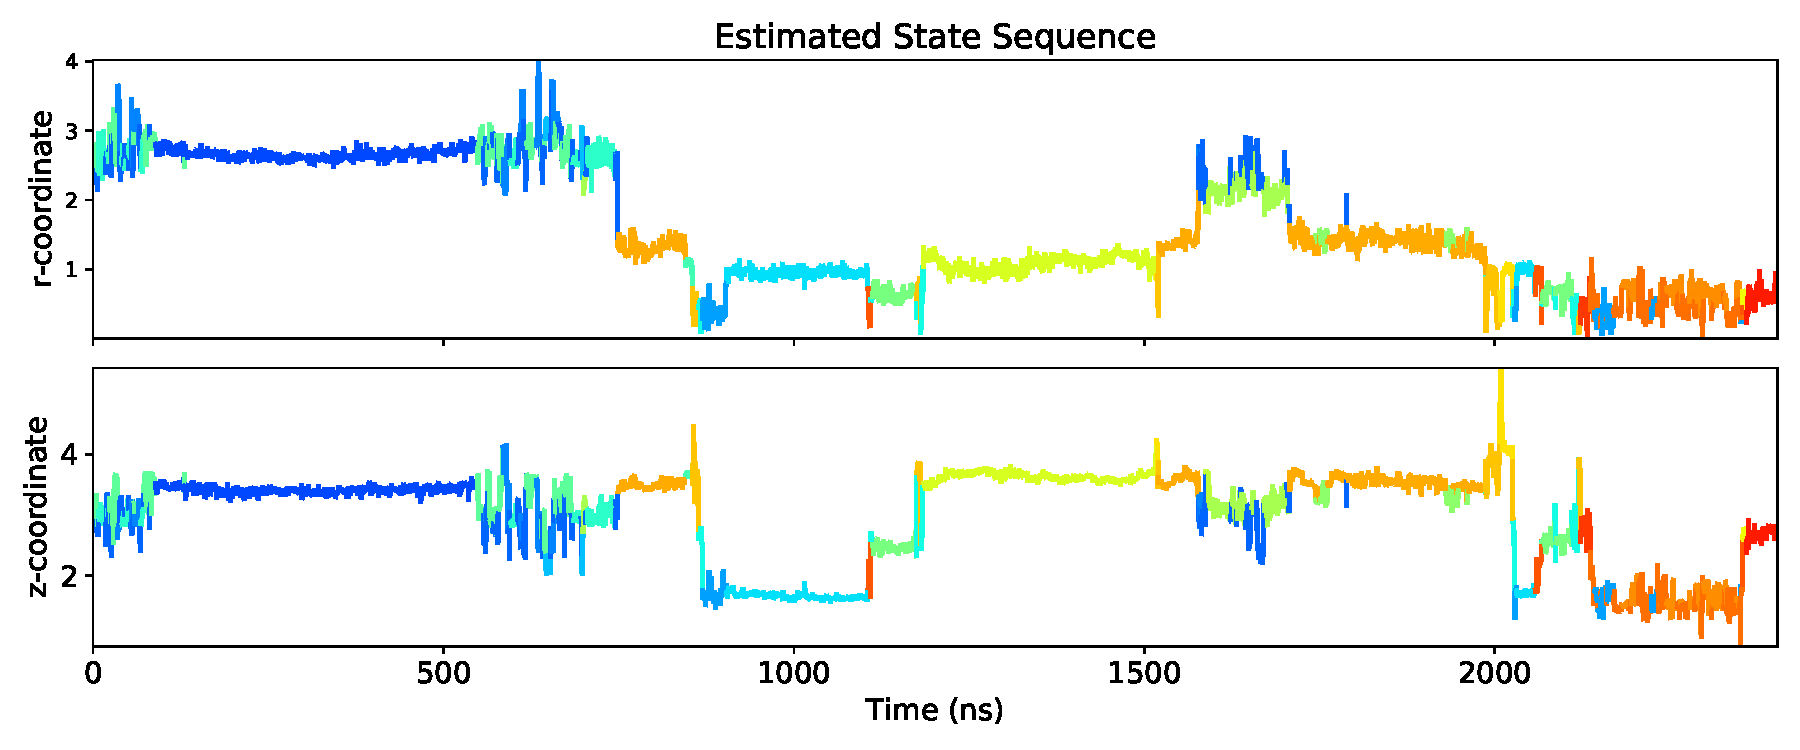
\includegraphics[width=\textwidth]{rz_unclustered_MET.pdf}
  \caption{The HDP-AR-HMM found 20 distinct VAR(1) states in this representative methanol trajectory.
  We performed the parameterization in 3D Cartesian coordinates, but for this figure, we 
  converted to cylindrical coordinates, with $r$ the distance from the pore center, to 
  provide a clearer picture of solute motion.}\label{fig:rz_unclustered}
  \end{figure}
  
  \subsection{Reproducing MD Trajectories and MSDs with the HDP-AR-HMM}\label{section:unclustered_MSD_prediction}

  Before analyzing solute behavior characteristic to the states identified by the
  HDP-AR-HMM, it is important to verify whether the state dynamics are consistent with MD
  both qualitatively and quantitatively. Therefore, we generated stochastic 
  realizations based on the parameters of each trajectory as described in 
  Section~\ref{method:realizations}.
  
  As shown in Figure~\ref{fig:qualitative_unclustered}, realizations of our model 
  produce trajectories with hopping and trapping behavior that is qualitatively 
  similar to the MD trajectories to which they were fit. It is important that our
  model reproduces this behavior so that we can have confidence in its potential
  usefulness for more quantitative predictions.
  
  \begin{figure}
  \centering
  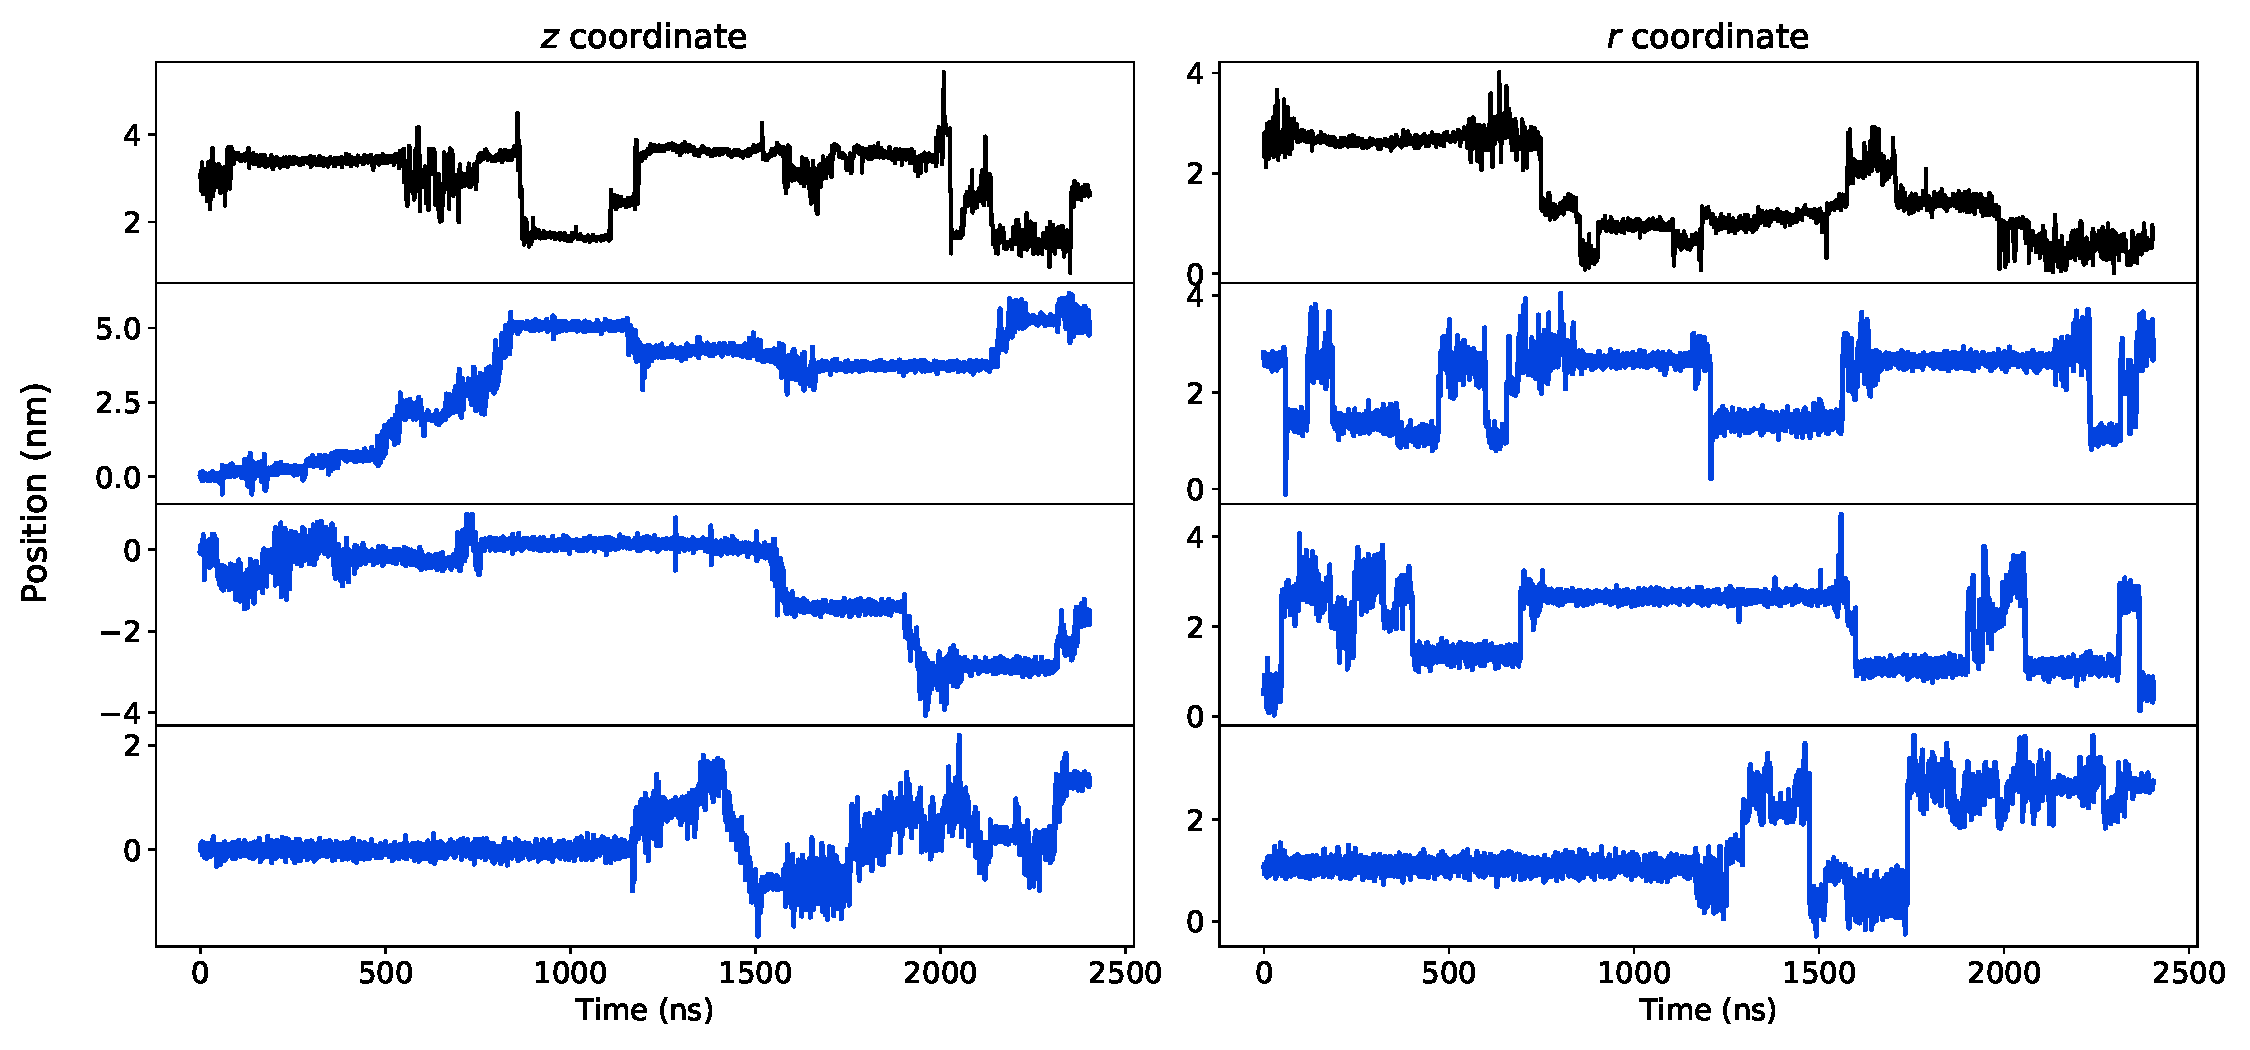
\includegraphics[width=\textwidth]{qualitative_unclustered_MET2.pdf}
  \caption{We used the parameters of the HDP-AR-HMM, whose state segments are 
  visualized in Figure~\ref{fig:rz_unclustered}, in order to construct an 
  ensemble of characteristic trajectories. The stochastic trajectories 
  generated by the parameters of the HDP-AR-HMM (blue) show similar hopping
  and trapping behavior exhibited by MD (black).
  }\label{fig:qualitative_unclustered}
  \end{figure}
  
  In Figure~\ref{fig:unclustered_msds}, we show that in most cases we can 
  reproduce the magnitude of the MD MSDs on long timescales within uncertainty
  using realizations of the HDP-AR-HMM. We generated the MSD curves using Method
  1 described in Section~\ref{method:realizations} of the methods. Our ability
  to reproduce the MSDs with stochastic models learned from the trajectories gives us confidence in their long term predictions.
  We underestimate the MSD of urea because of a small number of MD trajectories
  with uncharacteristically high MSDs. Despite our best efforts, we could not 
  adequately parameterize an HDP-AR-HMM which reproduced the uncharacteristic
  behavior (see Section~\ref{S-section:urea_underestimate} of the Supporting Information).
  On long time scales, the model's MSD appear to have a slope similar to the MD 
  MSD.

  A potential shortcoming of the HDP-AR-HMM applied to MD simulations is its 
  inability to reproduce the short time scale MSD curves. The MSDs predicted
  by the model tend to enter a linear regime much more quickly than the MD MSDs
  (see Figure~\ref{S-fig:unclustered_msd_shortlag} of the Supporting Information
  for example). This is not a major concern for predicting macroscopic properties
  since we are primarily interested in reproducing the MSDs on much longer 
  timescales.
  
  \begin{figure}
  \centering
  \begin{subfigure}{0.24\textwidth}
  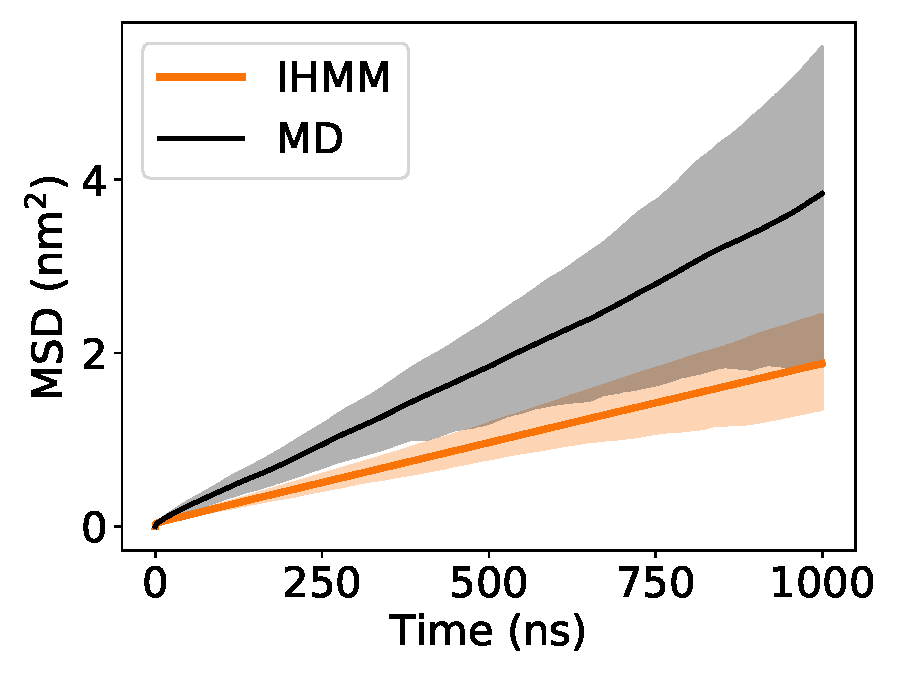
\includegraphics[width=\textwidth]{unclustered_msd_MET.pdf}
  \caption{methanol}\label{fig:unclustered_msd_MET}
  \end{subfigure}
  \begin{subfigure}{0.24\textwidth}
  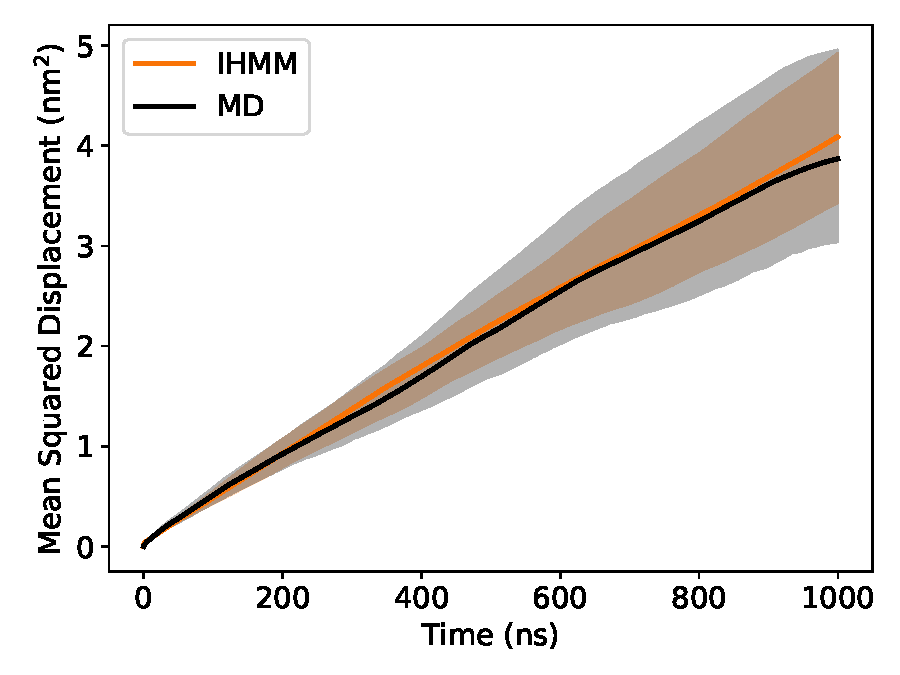
\includegraphics[width=\textwidth]{unclustered_msd_GCL.pdf}
  \caption{ethylene glycol}\label{fig:unclustered_msd_GCL}
  \end{subfigure}
  \begin{subfigure}{0.24\textwidth}
  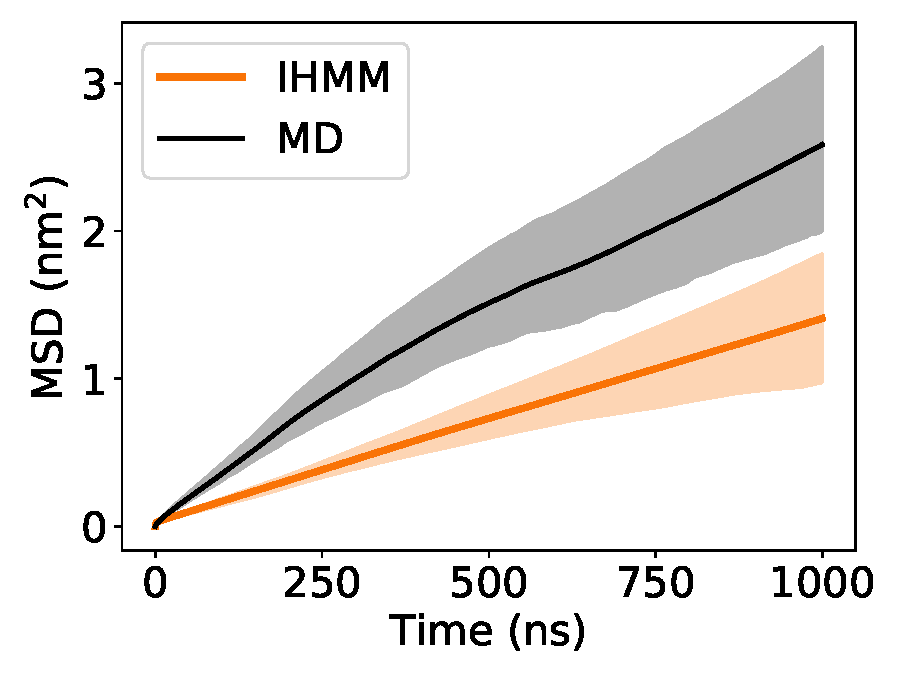
\includegraphics[width=\textwidth]{unclustered_msd_URE.pdf}
  \caption{urea}\label{fig:unclustered_msd_URE}
  \end{subfigure}
  \begin{subfigure}{0.24\textwidth}
  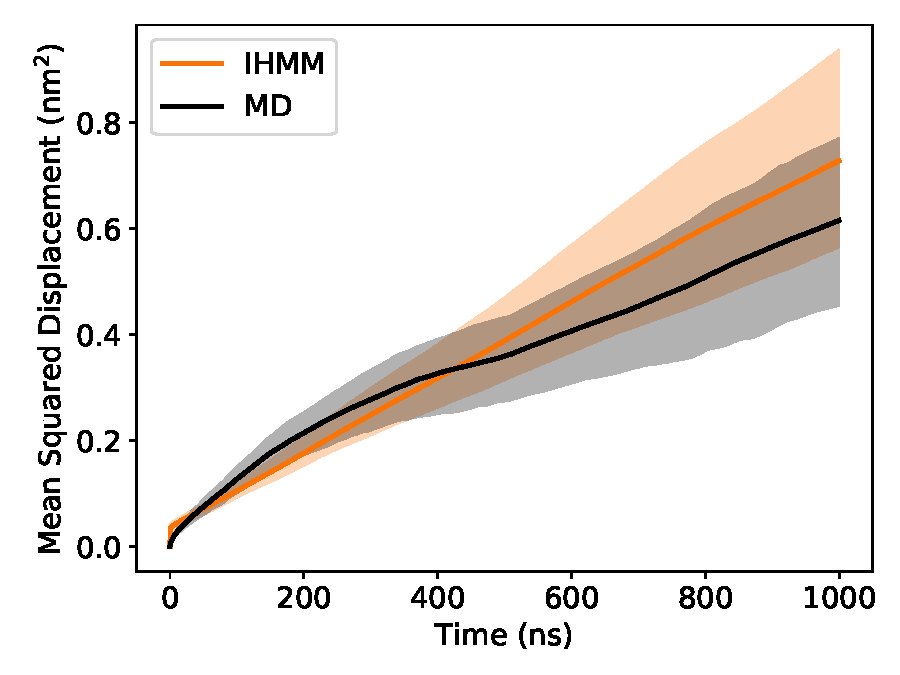
\includegraphics[width=\textwidth]{unclustered_msd_ACH.pdf}
  \caption{acetic acid}\label{fig:unclustered_msd_ACH}
  \end{subfigure}
  \caption{For methanol, ethylene glycol and acetic acid, the MD MSDs (black) and
  the MSDs calculated from realizations of the HDP-AR-HMM (orange) match within 
  uncertainty. The MD MSD of urea is under-predicted by the HDP-AR-HMM.
  }\label{fig:unclustered_msds}
  \end{figure}
  
  \subsection{Using HDP-AR-HMM Parameters to Predict Selectivity}\label{section:macroscopic_properties}
  
  Since we can generate trajectories that share the qualitative and quantitative
  features of our MD simulations, we can use realizations of the HDP-AR-HMM
  in order to estimate selectivity as described in Section~\ref{method:selectivity}.
  In Figure~\ref{fig:selectivity}, we plot the selectivities estimated by our
  models for all possible pairs of solutes.
  
  % BJC: Note that this figure is not finalized. It just takes a while to make 
  % because of bootstrapping and I keep forgetting to let it run overnight. I 
  % actually did it once, but had set save=False in the function I used in a jupyter notebook
  % In its final form, the errorbars will get smaller, and the means don't change by much.
  \begin{figure}
  \centering
  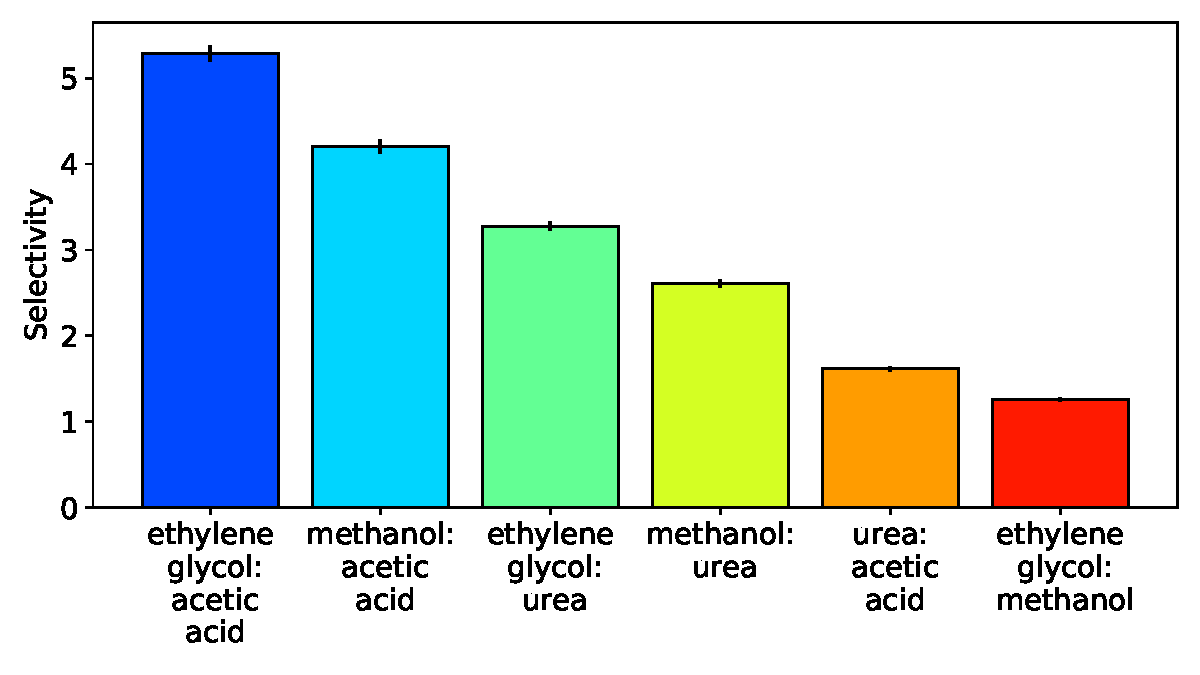
\includegraphics[width=0.6\textwidth]{selectivity2.pdf}
  \caption{Of the solutes studied, the models predict that the current generation 
  of H\textsubscript{II} LLC membranes may have the most success selectively removing 
  acetic acid and, to a lesser extent, urea from solution containing either ethylene
  glycol or methanol.
  }\label{fig:selectivity}
  \end{figure}

  The data suggests that the particular LLC membrane studied in this work, 
  up to the resolution of the molecular modeling, is capable of selectively 
  separating urea and acetic acid from ethylene glycol and methanol. Ethylene 
  glycol and methanol have comparable diffusivities while urea and acetic 
  acid have much lower diffusivities. 

  If we can understand the mechanisms that lead to the various observed transport
  rates, one may be able to redesign the LLC monomers in order to influence solute
  selectivities. For example, it is not obvious why ethylene glycol and methanol
  have similar transport rates. Ethylene glycol is a larger molecule with a 
  molecular weight about twice that of methanol. Their relative diffusivities are 
  not consistent with the inverse molecular size relationship implied by the 
  Stokes-Einstein equation.~\cite{gierer_molekulare_1953} The HDP-AR-HMM may 
  help us pinpoint the differences in their transport behavior.
  
  \subsection{Learning Mechanisms from the HDP-AR-HMM}\label{section:mechanisms}
  
  Solutes in this system show a wide range of behavior influenced by the 
  heterogeneity of the membrane's nanostructure as well as the interactions 
  between monomer and solute chemical functionality. Our application of the 
  HDP-AR-HMM can identify and distinguish these behaviors. The following approach 
  to analysis demonstrates how one can discover and explain the very complex
  behavior exhibited by solutes over long MD trajectories in terms of 
  solute-membrane interactions.
  
  \textit{State Clustering}: In order to reduce the state space to a more 
  manageable size, and to allow different solute trajectories to share 
  similar behavior, we clustered the states identified by the HDP-AR-HMM for each
  solute as described in Section~\ref{method:clustering}. In 
  Figure~\ref{fig:clustered_traj_MET}, we show the results of clustering on the 
  same methanol trajectory from Figure~\ref{fig:rz_unclustered}. Based on 
  the criteria described in Section~\ref{method:clustering},
  we chose to reducing the total state space for methanol from 287 to \nclusters. 
  
  Our goal is to derive the simplest model which adequately distinguishes
  different types of solute motion. By working to understand the parameters of 
  each cluster, we can uncover the associated transport mechanisms responsible
  for those parameters.
  
  \begin{figure}
  \centering
  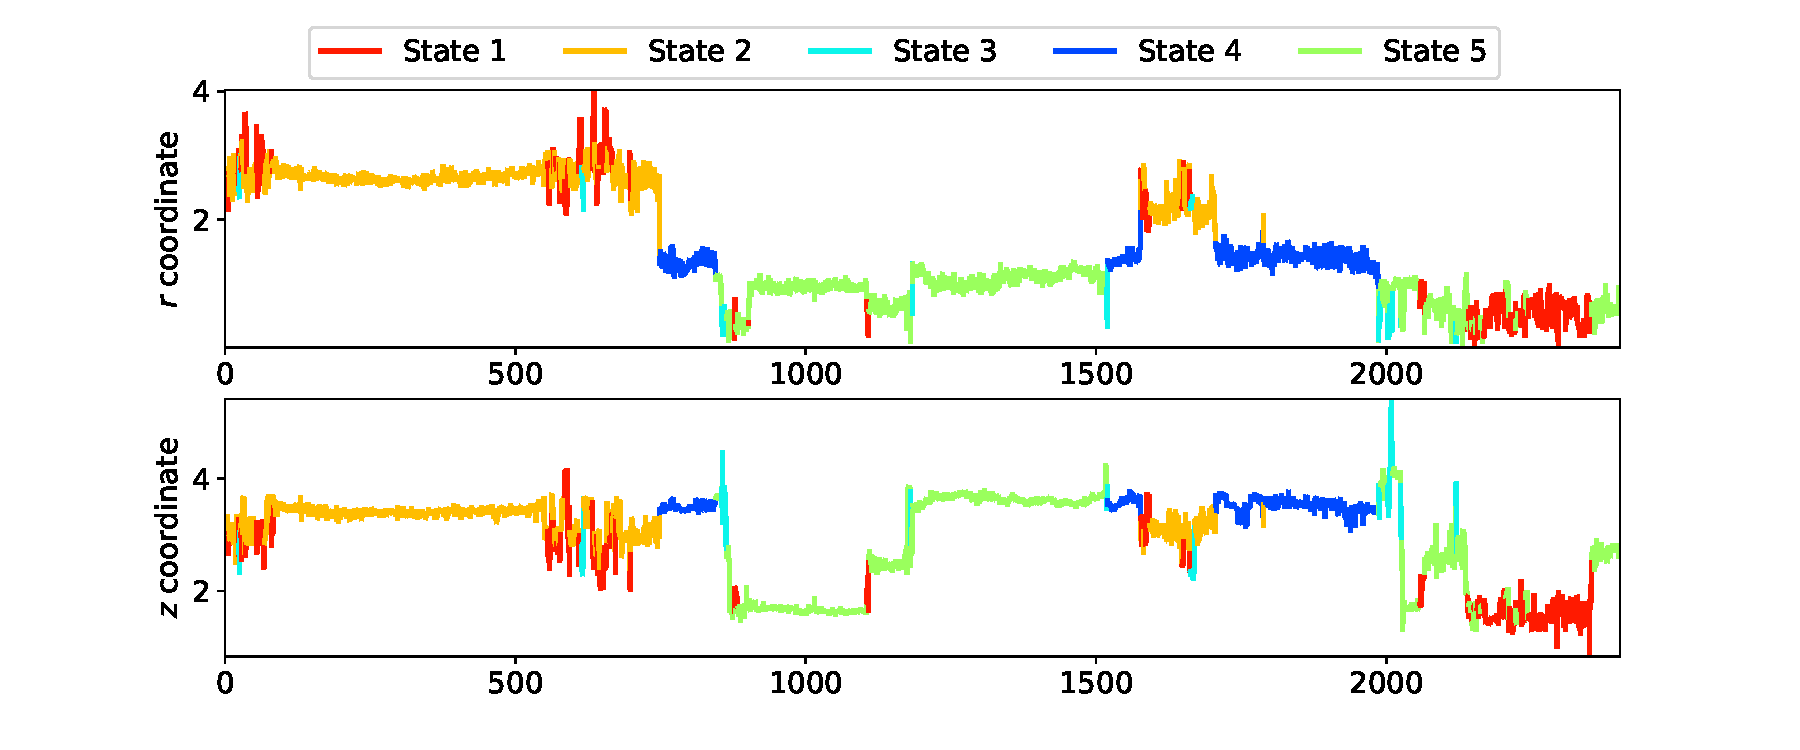
\includegraphics[width=\textwidth]{clustered_traj_MET_ward_10.pdf}
  \caption{We reduced the total state space from 287 to 10 total states 
  shared across all trajectories. For the trajectory in this figure, we reduced
  the total number of states from 20 (see Figure~\ref{fig:rz_unclustered}) to
  5.}\label{fig:clustered_traj_MET}
  \end{figure}
  
  \textit{Dynamics of clustered parameter sets}: The clustered
  parameter sets allow transitions between dynamics exhibited by the
  same solute from independent trajectories. This allows us to create
  hybrid trajectories which draw on dynamics of all the solutes
  simultaneously.
  
  Realizations based on the 10 clustered parameter sets do not show the same
  qualitative dynamics as the MD simulation trajectories. In 
  Figure~\ref{fig:qualitative_clustered_MET}, we compare MD trajectories to 
  realizations of our model using the clustered parameter sets. They lack the
  diversity of behavior which we see in the MD simulation trajectories, in particular, 
  they do not show the same range of trapping times and hop lengths. If we use
  a higher number of clusters, the qualitative match improves, but at the cost
  of a larger state space to interpret (see Section~\ref{S-section:qualitative}
  of the Supporting Information).
  
  In addition to qualitative mismatches, realizations of the clustered HDP-AR-HMM 
  under-predict the unclustered MSD predictions and the MD MSD. Much of a solute's 
  MSD is likely a consequence of short-lived trapping states with high variances.
  When clustering, disjoint segments with similar enough parameters are re-parameterized
  together as part of the same state, lengthening the lifetimes of very short-lived 
  states and suppressing the fluctuations of high variance states. In 
  Figure~\ref{fig:clustered_MSD}, it is evident that increasing the number of clusters
  increases the predicted MSD. Matching the unclustered MSDs would likely require many
  more clusters, at which point the benefits of clustering are lost. 
  
  \begin{figure}
  \centering
  \begin{subfigure}{0.63\textwidth}
  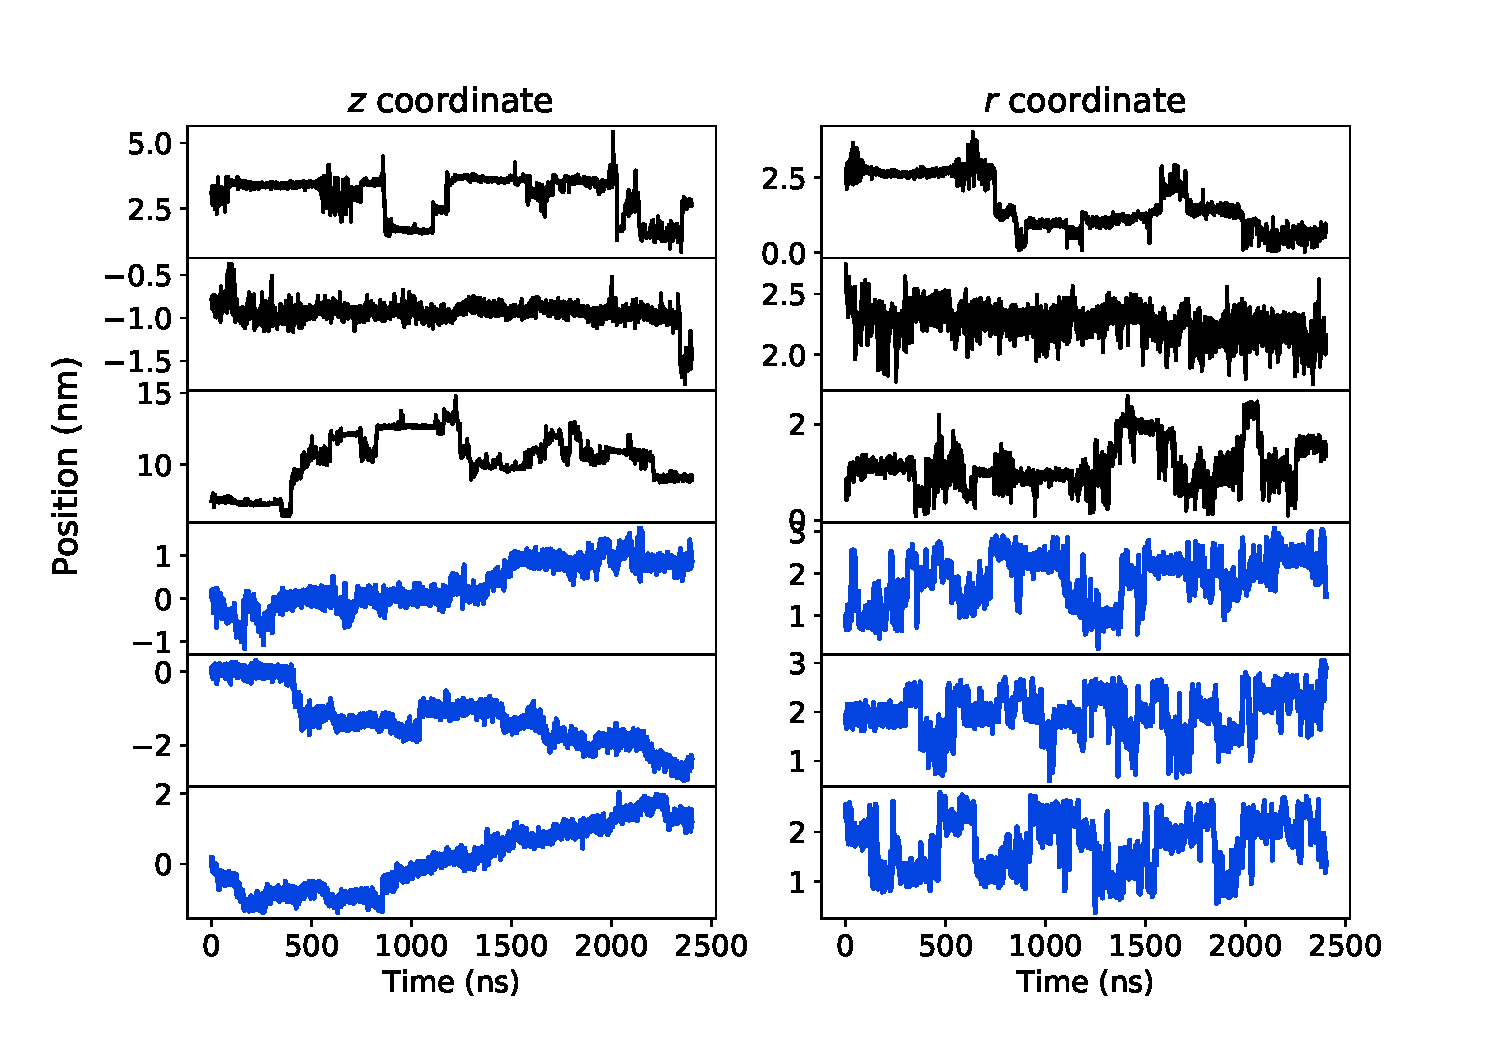
\includegraphics[width=\textwidth]{qualitative_clustered_MET_10.pdf}
  \caption{}\label{fig:qualitative_clustered_MET}
  \end{subfigure}
  \begin{subfigure}{0.35\textwidth}
  \vspace{2.25em}
  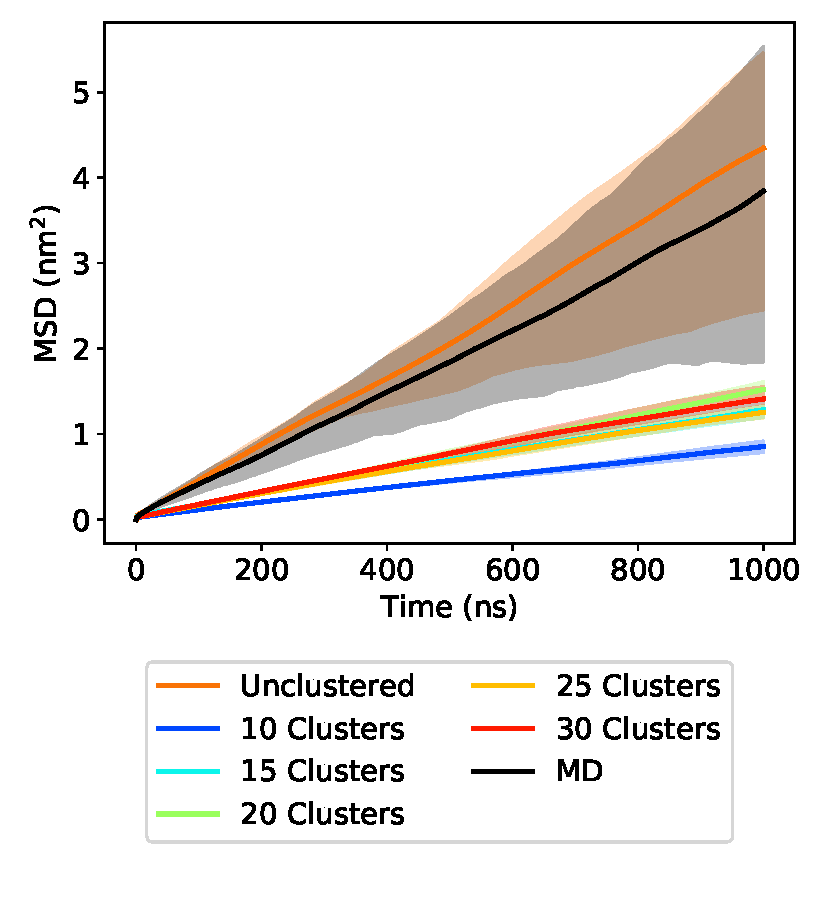
\includegraphics[width=\textwidth]{msd_nclusters.pdf}
  \caption{}\label{fig:clustered_MSD}
  \end{subfigure}
  \caption{(a) Stochastic trajectory realizations generated from our model 
  (blue) based on the 10 clustered methanol parameter sets do not qualitatively
  reproduce the diversity of behavior seen in our MD trajectories (black). 
  (b) MSD predictions by clustered parameter sets consistently under-predict 
  the MD MSD. They appear to do a better job of predicting MSDs as the number
  of clusters increases.}\label{fig:clustered_dynamics}
  \end{figure}
  
  It is possible that we could improve the MSD predictions generated by the 
  clustered parameter sets by modifying the transformations made to the
  unclustered parameters. For example, it maybe possible to rescale the
  parameters in order to better distinguish states with long dwell times
  and high variance when clustering. However, we did not pursue this too 
  far in order to avoid over-fitting the data.

  \textit{The dynamics of frequently occurring states}: We may learn the most by 
  studying the dynamical modes common to the majority of methanol trajectories.
  Of the 10 state clusters, only 5 are sampled by a significant number of 
  trajectories (Figure~\ref{fig:prevalence}). All of which are present in 
  Figure~\ref{fig:clustered_traj_MET}.
  
  \begin{figure}
  \centering
  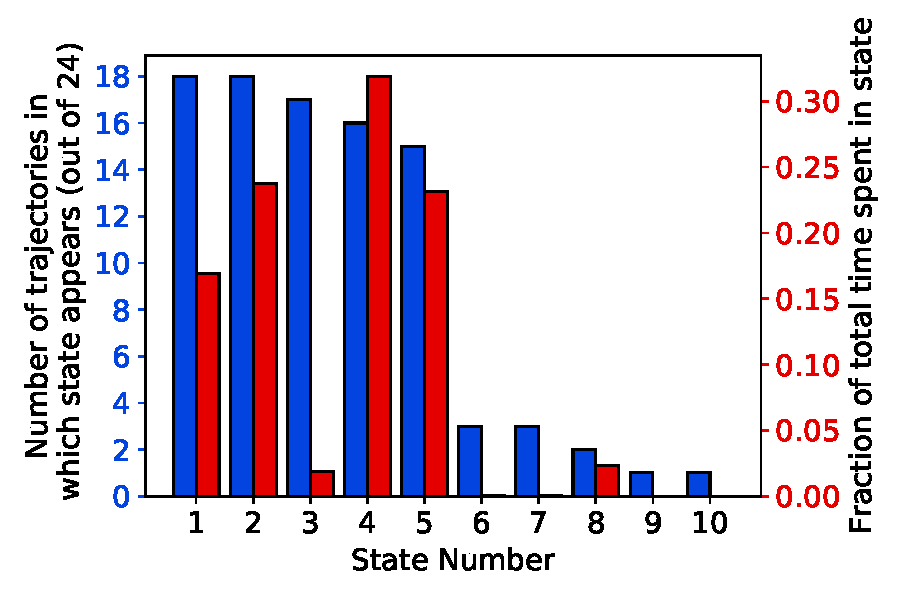
\includegraphics[width=0.5\textwidth]{prevalence.pdf}
  \caption{5 out of the 10 clustered states are visited by 15 or more of the methanol
  trajectories (States 1--5). Although a majority of the solutes visit these 5 
  predominant states, the amount of time spent in each varies widely. For example, methanol
  does not spend a significant amount of time in State 3 because, as discussed later, it 
  is a short-lived state. We still consider State 3 as a predominant state because it
  is may be a significant contributer to solute MSD.
  }
  \label{fig:prevalence}
  \end{figure}
  
  The parameters of the five predominant states provide clues about the associated solute
  behavior. Characteristic dynamics of the following states appear in 
  Figure~\ref{fig:clustered_traj_MET}. A more in-depth analysis of the state parameters
  is given in Section~\ref{S-section:clustered_parmeters} of the Supporting Information.
  \begin{enumerate}[label={State \theenumi :}, leftmargin=3.5\parindent]
  
     \item This state has intermediate dwell times with high past-hop dependence (large
     entries of $A$). The cluster's radial mean is 1.5 nm which is about halfway between
     the pore center and tail ends. Evidence from Figure~\ref{fig:clustered_traj_MET} 
     suggests that this state occurs essentially evenly across possible radial
     distances from the pore center.
     
     \item This state's radial mean of 2.4 nm implies that it occurs exclusively in the
     tail region. Its fluctuations are small and there is little past hop dependence.
     
     \item This is likely a hopping state that strongly contributes to the solute's MSD. 
     It is short lived and has large fluctuations which often results in very large hops.
     Like state 1, we see this type of behavior near the pore center and near the ends of the tails.
     
     \item This is a trapping state, having the longest expected dwell time among the predominant
     states, with a strong dependence on its previous fluctuation. Evidence from 
     Figure~\ref{fig:clustered_traj_MET} and a radial mean of 1.8 nm suggest that 
     it tends to occur at intermediate distances from the pore center with perhaps
     a higher tendency to occur deeper within the tails.
     
     \item This is an intermediate-length trapping state that occurs 0.9 nm from the pore 
     center on average. Fluctuations are small and relatively independent of its previous 
     fluctuation.
     
  \end{enumerate}
   
  \textit{Relating Parameters to Solute-Membrane Interactions}: Based on the
  molecules and ions which constitute this system, it is logical to search for hydrogen 
  bonding interactions and electrostatic association with sodium ions. All of 
  the solutes are polar and have hydrogen bond donating and accepting groups. The monomers 
  have 10 oxygen atoms distributed from head to tail that are capable of 
  accepting hydrogen bonds. The ionic bond between the head groups and sodium ions 
  can be easily broken since both components can be stabilized by surrounding 
  water molecules and solutes 

  For methanol, hydrogen bonding is a much more dominant interaction than association
  with sodium ions. In Figure~\ref{fig:hbond_fractions}, we show that methanol 
  participates in hydrogen bonds to various parts of the monomer between 27 and
  45\% of the total time it occupies the predominant states. Methanol associates 
  with sodium ions less than 10\% of its time and for relatively short periods 
  of time while in predominant states. 

  The distribution of types of hydrogen bonds and associated hydrogen bond lifetimes
  varies by predominant state, as seen in more detail in Figure~\ref{fig:hydrogen_bonding}.
  \begin{itemize}
	\item States 1 and 2 primarily have hydrogen bonds to the ester groups at the ends
	of the monomer tails and, to a smaller extent, the ether linkages between the 
	monomer head group and tails. 
    \item State 1 methanol molecules that donate hydrogen bonds to the tail oxygen 
    atoms exhibit by far the longest hydrogen bond lifetimes among all states. 
    \item Methanol molecules in states 3 and 4 hydrogen bond to all regions of the
    monomer relatively evenly, which is consistent with our earlier observation that
    states 3 and 4 are representative of behavior seen radially throughout the membrane
    pores. 
    \item State 3 has the lowest hydrogen bond and sodium association lifetimes which
    is consistent with its short dwell times. These are fleeting interactions since it
    is likely a high variance transitory state. 
    \item Finally, methanol molecules in state 5 hydrogen bond almost exclusively 
    to the carboxylate head groups and ether linkages which is consistent with the 
    low (close to the pore center) radial mean of the cluster.
  \end{itemize}

  \begin{figure}
  \centering
  \begin{subfigure}{0.475\textwidth}
  \centering
  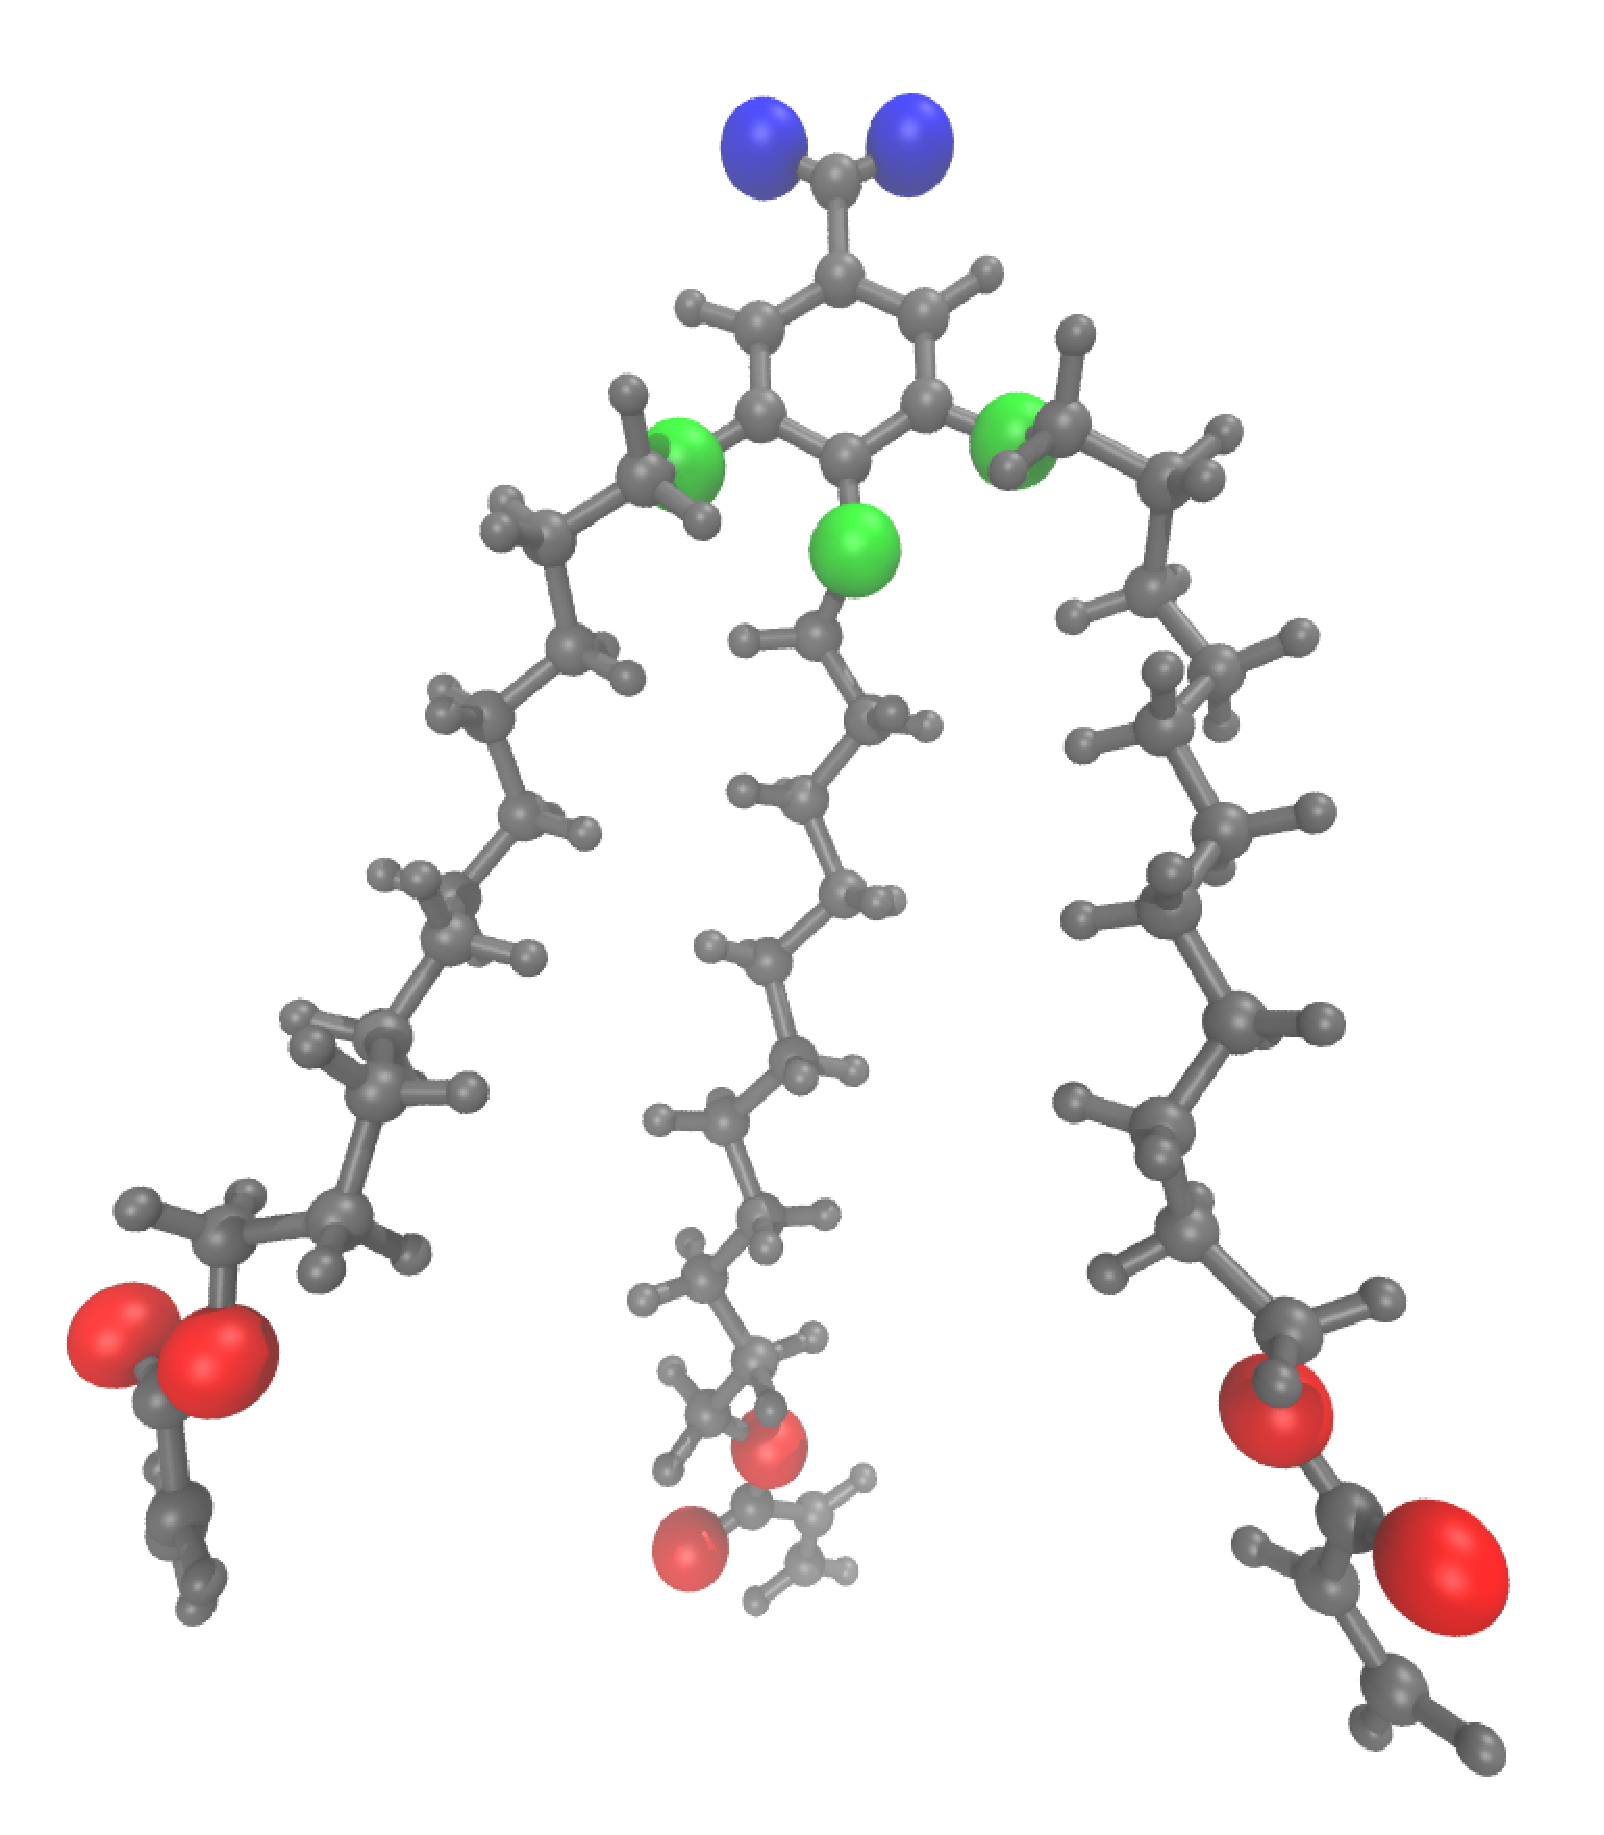
\includegraphics[width=0.6\textwidth, angle=0]{monomer_oxygens.pdf}
  \caption{}\label{fig:monomer_oxygens}
  \end{subfigure}
  \begin{subfigure}{0.475\textwidth}
  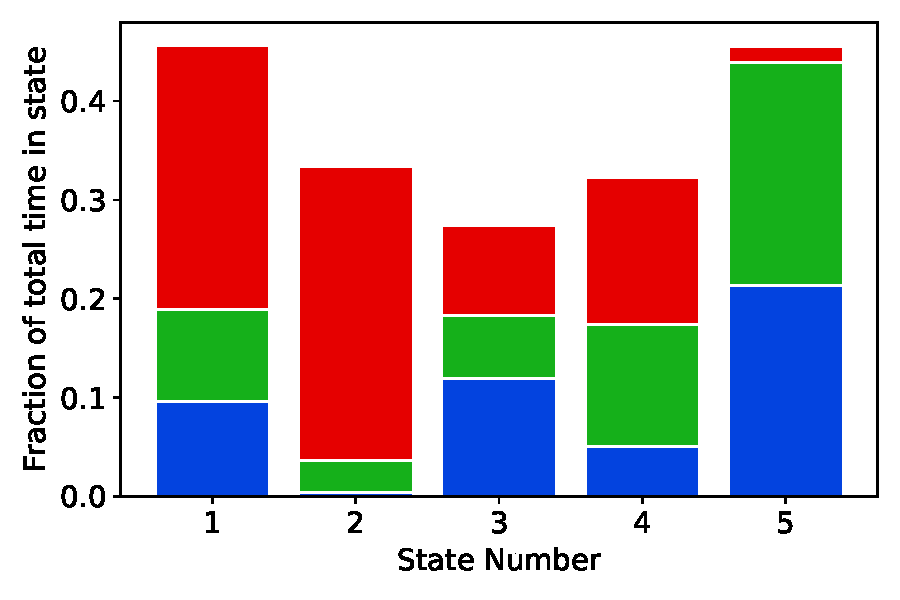
\includegraphics[width=\textwidth]{hbond_fractions.pdf}
  \caption{}\label{fig:hbond_fractions}
  \end{subfigure}
  \begin{subfigure}{0.475\textwidth}
  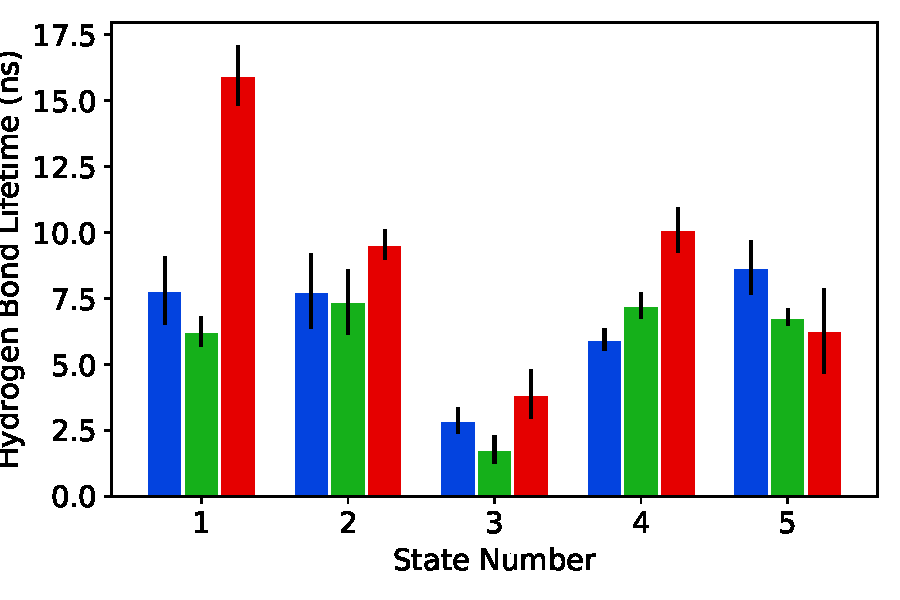
\includegraphics[width=\textwidth]{hbond_lifetimes.pdf}
  \caption{}\label{fig:hbond_lifetimes}
  \end{subfigure}
  \begin{subfigure}{0.475\textwidth}
  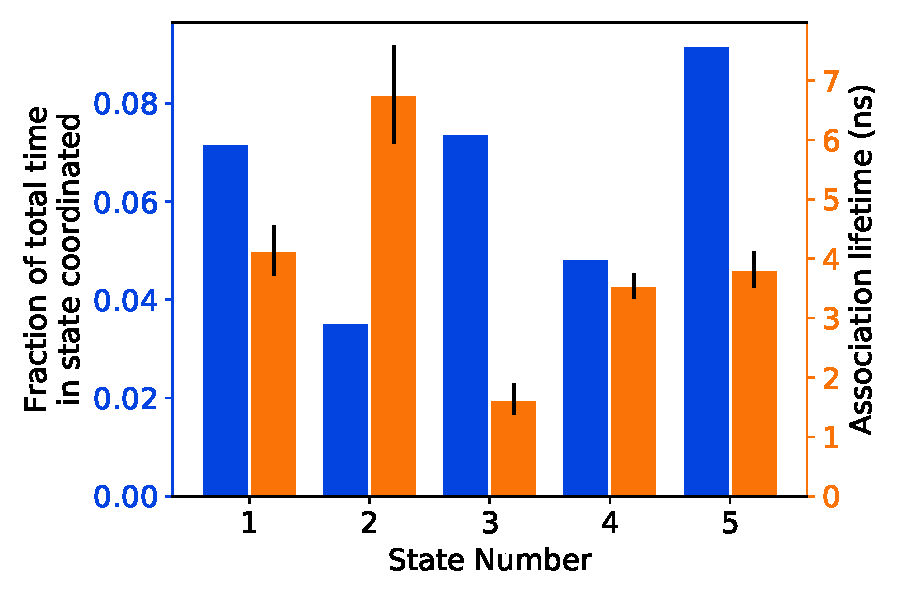
\includegraphics[width=\textwidth]{association_fraction_lifetimes.pdf}
  \caption{}\label{fig:association_fraction_lifetimes}
  \end{subfigure}
  %y-axis label being cut off?
  \caption{(a) We analyzed hydrogen bonds donated by methanol to the highlighted oxygen
  atoms in three regions of the monomer: the carboxylate groups (blue), the ether linkages
  (green) and the tails (red). (b) For each predominant state (states 1--5 described in 
  Figure~\ref{fig:prevalence}), we plotted the fraction of the total time in that state 
  spent hydrogen bonding to various regions of the monomer, color coded to match (a).
  (c) For each type of hydrogen bond in each predominant state, we calculated the 95th percentile
  of hydrogen bond lifetimes. (d) We also analyzed the frequency and lifetimes of solute 
  association with sodium ions. Methanol associates with sodium less than 10\% of the total 
  time it occupies any of the predominant states.
  }
  \label{fig:hydrogen_bonding}
  \end{figure}
  
  \textit{Comparison of Solute Behavior}: We can apply a similar analysis to the other 
  solutes in this study and learn new information by comparing their behavior. 
  Where referenced in the following analysis, we define the predominant states 
  exhibited by each solute as any state visited by at least half (12) of the 
  solute trajectories. By our definition and based on our choice to study 10 
  clusters for each solute, methanol, ethylene glycol, urea and acetic acid are
  characterized by 5, 6, 5 and 4 predominant states respectively 
  (see Figure~\ref{S-fig:state_prevalence} of the Supporting Information).
 
  The size and chemical functionality of the solutes dictates the interactions which
  influence solute transport. Figure~\ref{fig:hbonds_assoc_summary} shows that the
  solutes donate hydrogen bonds and associate with sodium ions to varying degrees.
  In fact methanol interacts the least by these mechanisms by far. This is likely 
  because methanol is very small and it is easier for it to partition into the tail
  region where there are fewer groups with which it can interact (see Figure~\ref{fig:rdf_summary}).
  Acetic acid, urea and ethylene glycol are slightly larger than methanol and contain 
  multiple polar substituents which stabilize them closer to the pore center.
  These three solutes also participate in significantly more sodium ion association. 
  In our previous work, we showed that sodium ions frequently associate with the 
  carbonyl groups of acetic acid and urea because the carbonyl oxygen atoms are
  unshielded and have a relatively high partial negative charge.~\cite{coscia_chemically_2019}
  
  \begin{figure}
  \centering
  \begin{subfigure}{0.49\textwidth}
  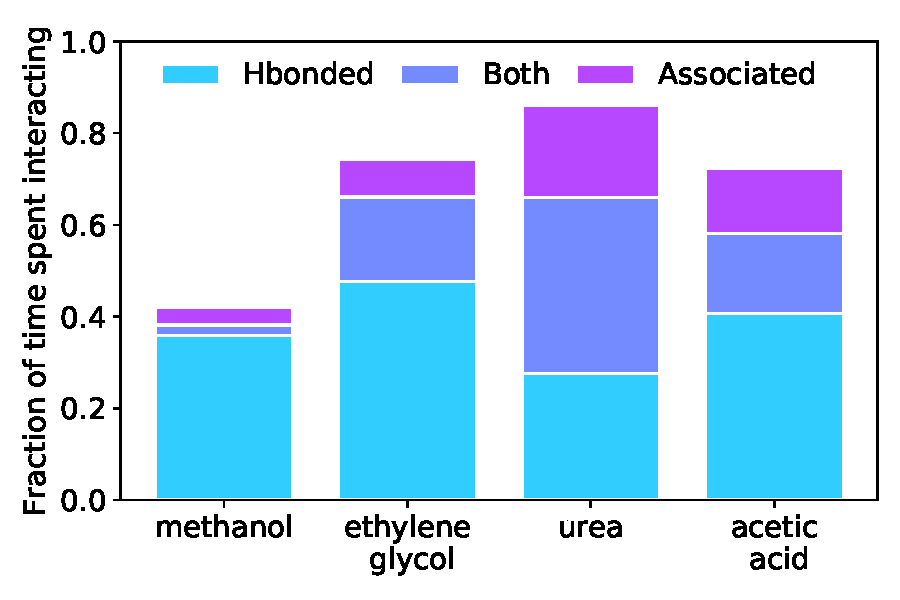
\includegraphics[width=\textwidth]{hbonds_assoc_summary.pdf}
  \caption{}\label{fig:hbonds_assoc_summary}
  \end{subfigure}
  \begin{subfigure}{0.49\textwidth}
  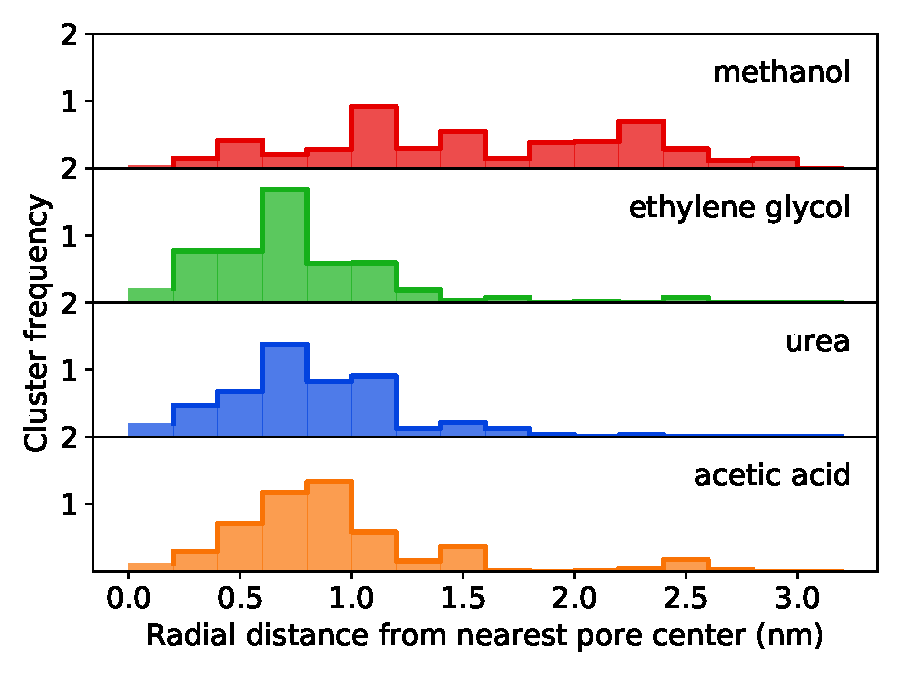
\includegraphics[width=\textwidth]{rdf_summary.pdf}
  \caption{}\label{fig:rdf_summary}
  \end{subfigure}
  \begin{subfigure}{0.49\textwidth}
  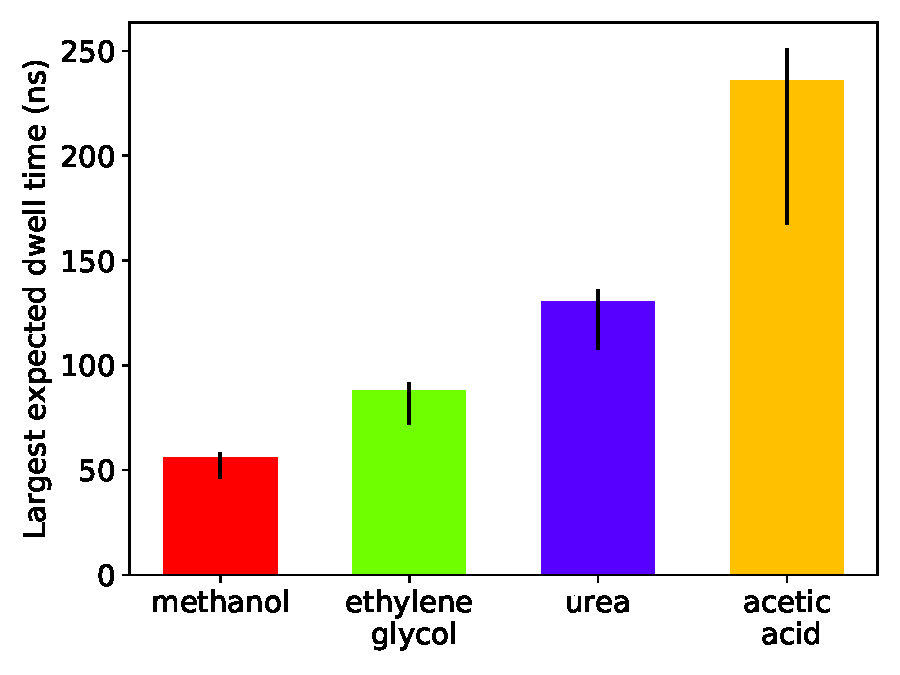
\includegraphics[width=\textwidth]{dwell_time_summary.pdf}
  \caption{}\label{fig:dwell_time_summary}
  \end{subfigure}
  \begin{subfigure}{0.49\textwidth}
  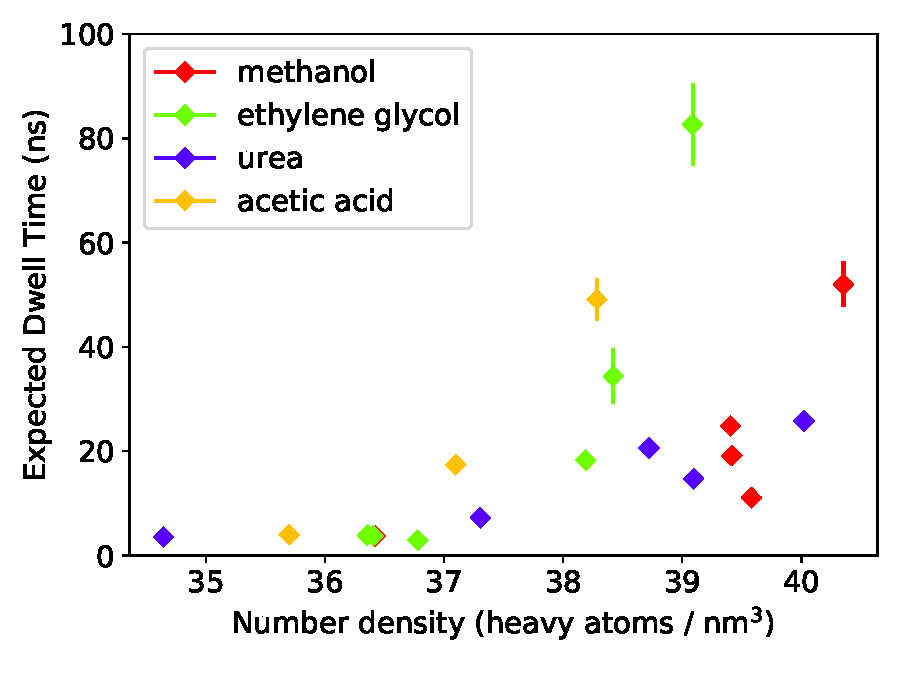
\includegraphics[width=\textwidth]{density_comparison.pdf}
  \caption{}\label{fig:density_comparison}
  \end{subfigure}
  \caption{(a) Solutes hydrogen bond and associate with sodium ions
  to different degrees. Sometimes, they participate in both interactions at
  once. (b) The radial means of the unclustered states weighted
  by the length of time spent in that state. Most solutes spend the majority of
  their time close to the pore center. Only methanol has a significant density
  far from the pore center. (c) The 95\textsuperscript{th} percentile of dwell
  times, collected by measuring the length of each disjoint segment according 
  to the clustered state sequences, is inversely related to the solute MSDs.
  (d) The expected dwell time of solutes increases in states with high local 
  number density of surrounding heavy atoms.
  }\label{fig:summaries}
  \end{figure}
  
  Solutes which experience longer dwell times tend to have lower MSDs. 
  In Figure~\ref{fig:dwell_time_summary}, we plot the 95\textsuperscript{th}
  percentile of dwell times for each solute. The evidence suggests that the 
  long time scale MSDs (we use the MSDs after a 1000 ns time lag in Figure~\ref{fig:dwell_time_summary})
  are inversely related to dwell times. Both acetic acid and urea participate 
  in many hydrogen bonds and sodium ion association interactions and the states
  visited by both solutes have similar distributions of radial means, but
  acetic acid has much longer dwell times, and hence a lower MSD. 
  This may be because acetic acid is a stronger hydrogen bond donor than urea.
  
  In addition to hydrogen bonding and sodium ion association, the local density 
  of heavy atoms experienced by each solute may play a large role in the length
  of solute entrapment. In Figure~\ref{fig:density_comparison}, we show that the
  expected dwell time (see Equation~\ref{eqn:dwell_times}) of solutes in 
  predominant states tends to increase with the local density of surrounding 
  heavy atoms. High local density combined with polar and electrostatic 
  interactions act cooperatively to keep solutes in place.
  
  \section{Conclusion}
  
  We have shown that the HDP-AR-HMM can be used to automatically parameterize solute 
  time series with an unknown number of latent dynamical modes. Initially, we applied
  the algorithm to each trajectory independently. Using the model parameters fit
  to each trajectory, we generated stochastic realizations of solute trajectories that
  can qualitatively and quantitatively reproduce the behavior of MD solute 
  trajectories. The realizations show the hopping and trapping behavior that is
  characteristic of polar solutes in this system. 
  
  By pooling MSDs predicted by models fit to each trajectory, we can reproduce
  the solute MSDs measured directly from our MD-simulated trajectories. 
  The low computational expense of generating these stochastic trajectories allows
  one to project solute behavior on much longer timescales, allowing us to predict
  selectivity, an experimentally-relevant quantity.
  
  In order to gain a mechanistic understanding of solute motion, we showed how 
  we could cluster the parameter sets in order to reduce the state space down
  to an interpretable size. We coupled analysis of the clustered parameter sets
  with measurements of membrane properties and solute-membrane interactions 
  in order to gain a detailed understanding of the diverse sets behavior 
  exhibited by solutes in these membranes. We showed how
  solute motion is influenced by hydrogen bonding, sodium ion association and local
  membrane density.
  
  When clustering, our goal was to create the simplest model possible that gave
  clear mechanistic insight. This is particularly important for systems where transport mechanisms
  are not easily hypothesized. However, once one gains some mechanistic understanding,
  as we have in this work, the clustering procedure can be modified in order to 
  study specific interactions or radially dependent behavior.
  
  Although we showcase this modeling approach by example, it is important to
  recognize the generality of this analysis, especially in the context of molecular
  simulations. Vector autoregressive models can describe a diverse set of behavior
  and so the HDP-AR-HMM may be suited to study many types of motion, including those not 
  characterized by hopping and trapping. The HDP-AR-HMM is a powerful approach for 
  understanding particle motion as well as for modeling long time scale trajectories
  which can give macroscopic insight.
  
  \section*{Supporting Information}

  Detailed explanations and expansions upon the results and procedures mentioned in
  the main text are available in the Supporting Information. 

  \section*{Acknowledgments}

  This work was supported in part by the ACS Petroleum Research Fund
  grant \#59814-ND7 and a Graduate Assistance in Areas of National Need (GAANN) 
  fellowship which is funded by the U.S. Department of Education. 
  Molecular simulations were performed using the Extreme Science and
  Engineering Discovery Environment (XSEDE), which is supported by National
  Science Foundation grant number ACI-1548562. Specifically, it used the Bridges
  system, which is supported by NSF award number ACI-1445606, at the Pittsburgh
  Supercomputing Center (PSC). This work also utilized the RMACC Summit supercomputer,
  which is supported by the National Science Foundation (awards ACI-1532235 and
  ACI-1532236), the University of Colorado Boulder, and Colorado State
  University. The Summit supercomputer is a joint effort of the University of
  Colorado Boulder and Colorado State University.

  \clearpage

  \bibliographystyle{ieeetr}
  \bibliography{hdphmm}
  
  \newpage

  \section*{TOC Graphic}
  
  \begin{figure}[!htb]
  \centering
  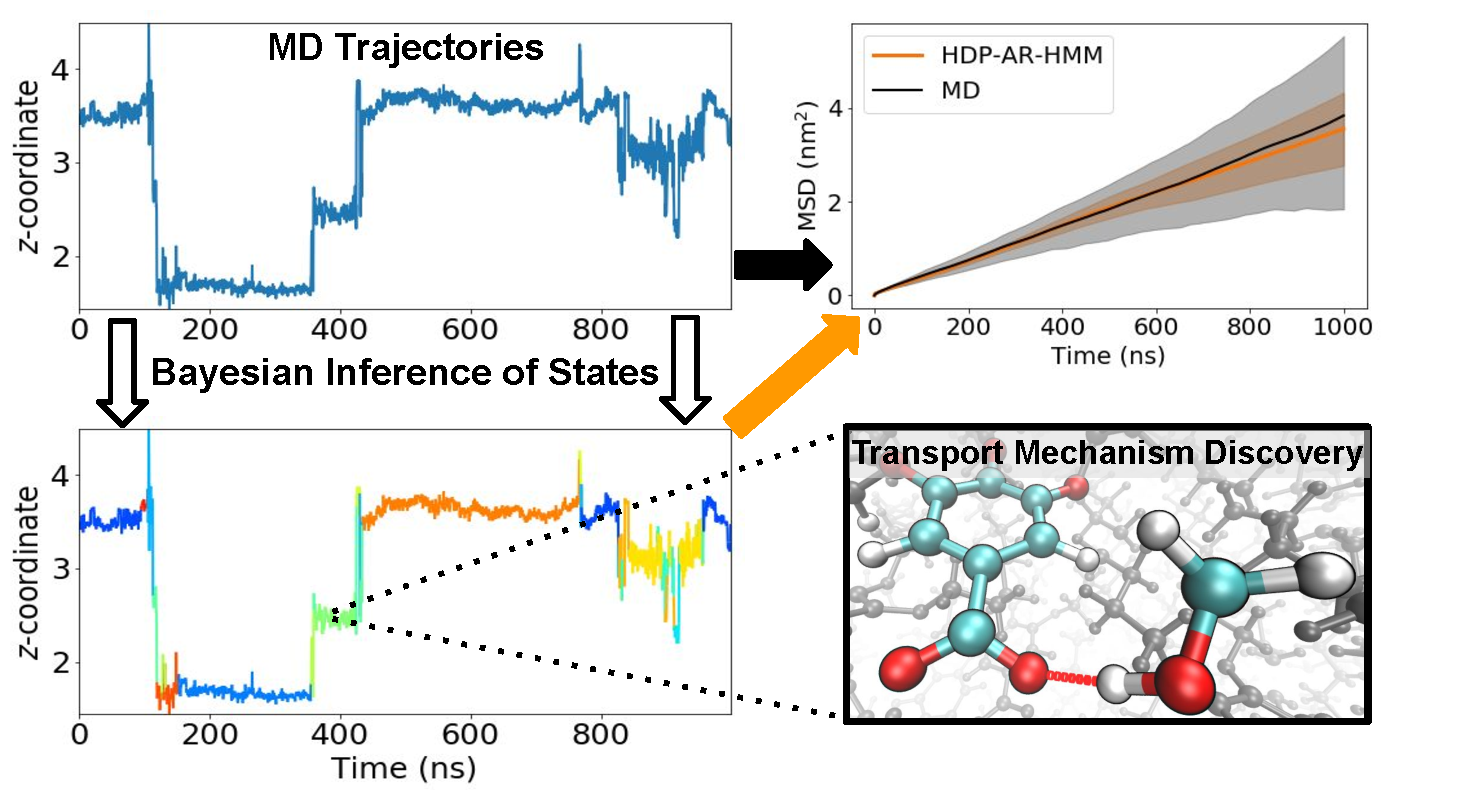
\includegraphics[width=3.25in]{hdphmm_TOC_v2.pdf}
  \end{figure}

\end{document}

% LocalWords:  BJC micropollutants Desalination permeability nanofiltration LLC
% LocalWords:  Amphiphilic nanostructures Lyotropic amphiphilic lyotropic MSDDM
% LocalWords:  solutes selectivities solute nanoscopic timescales MSDs MSD HMMs
% LocalWords:  nonparameteric Parrinello Rahman barostat rescale transitioning
% LocalWords:  al's HMM Dirichlet HDP DP Wishart TODO SI al MATLAB teh gael pdf
% LocalWords:  nonparametric bayesian solute's reparameterized intracluster ca
% LocalWords:  delocalize Luzar Chandler histogrammed interpolator methanol's
% LocalWords:  nanostructure carboxylate VMD nonidealities hbonds outlier GAANN
% LocalWords:  autogregressive PRF ACS XSEDE ACI HDP-AR-HMM nanoporous flowback evy
% LocalWords:  timescale subdiffusive coscia subdiffusion calderon GROMACS der
% LocalWords:  berendsen gromacs spoel hess emailed plateauing hmm ne gelman AR
% LocalWords:  walt numpy GCL URE ACH IMMM subsubsection modT convective vmd Na
% LocalWords:  scannable subsubcaptions errorbars uncharacteristicness facelift
% LocalWords:  PSC RMACC hdphmm TOC nominalizations dischinger ramaseshan Baum
% LocalWords:  functionalized teuerle jasra markov bioinformatics hughes yoon
% LocalWords:  hines diarization MJLSs MJLS SLDSs SLDS hamada jk params MNIW BP
% LocalWords:  plateaued nclusters leftmargin trans diffusivity sorption alkane
% LocalWords:  ness substituents desalination fonseca couto welch singhal noe
% LocalWords:  shirtsgroup superdiffusive diffusivities jazani wang persson CPC
% LocalWords:  shortlag jupyter ester
